\documentclass[12pt]{report}
%\documentclass{article}
\usepackage{uwmthesis}
\usepackage{amsmath,amsthm}
\usepackage{amssymb}
\usepackage{xcolor}
\usepackage{listings}
\usepackage{algorithm}
\usepackage[noend]{algpseudocode}
\usepackage{flexisym}
\usepackage{graphicx}
\usepackage{courier}
\usepackage{tikz}
\usepackage{pgfplots}
\pgfplotsset{width=6cm,compat=newest}

% "define" Scala
\lstdefinelanguage{scala}{
  morekeywords={abstract,case,catch,class,def,%
    do,else,extends,false,final,finally,%
    for,if,implicit,import,match,mixin,%
    new,null,object,override,package,%
    private,protected,requires,return,sealed,%
    super,this,throw,trait,true,try,%
    type,val,var,while,with,yield},
  otherkeywords={=>,<-,<\%,<:,>:,\#,@},
  sensitive=true,
  morecomment=[l]{//},
  morecomment=[n]{/*}{*/},
  morestring=[b]",
  morestring=[b]',
  morestring=[b]"""
}

\lstset{basicstyle=\footnotesize\ttfamily}
%\usepackage{titling}
\makeatletter
\def\tagform@#1{\maketag@@@{[\ignorespaces#1\unskip\@@italiccorr]}}
\makeatother

\begin{document}
\title{\textit{h}-CFA\@: A Simplified Approach for\\ Pushdown Control Flow Analysis}
\author{Fei Peng}
\Program{Computer Science}
\majorprof{Tian Zhao}
\degree{Master of Science}


%\maketitle
%\tableofcontents
\Abstract{
%\begin{abstract}
  In control flow analysis (CFA), call/return mismatch is always a problem that dramatically reduces analysis precision.
  Original \textit{k}-CFA uses bounded call strings to obtain limited call/return matching, but it has a serious performance problem
  due to its coupling of call/return matching with context-sensitivity of values.
  Meanwhile, abstracting abstract machine (AAM), a configurable framework for constructing abstract interpreters,
  introduced store-allocated continuation that made the soundness of abstract interpreters easily obtainable.
  Recently, there are three related approaches (PDCFA, AAC, and P4F) that provide call/return matching for AAM by modeling call-stack as a pushdown system.
  However, PDCFA needs significant engineering effort to implement.
  AAC incurs high overhead and is hard to understand while P4F cannot work with monovariant analysis (0-CFA).
  To overcome the above shortcomings, we developed a new method, \textit{h}-CFA, to address the call/return mismatch problem.
  Our method uses AAM and is very easy to implement for ANF style program.

  In addition, our method reveals an essential property of pushdown CFA,
  which we exploited in the development of a static analyzer for JavaScript, named JsCFA, without ANF transformation.
  JsCFA adopts a technique to solve the environment problem or fake rebinding, which eliminates more defects of monovariant analysis.
  This, in cooperation with exact call/return matching, yield more precise analysis and better performance.
  Moreover, JsCFA supports a configurable interface to add context-sensitivity to selected areas of programs.
  JsCFA applies the interface to improve the analysis precision for runtime object extensions.
  Finally, we quantitatively evaluated the performance of JsCFA\@.
%\end{abstract}
}

\beforepreface
%\prefacesection{Preface}
%This thesis tells you all you need to know about...
\afterpreface

\chapter{Introduction}
\label{Introduction}
%\section{Control Flow Analysis}
%\label{sub:CFA}
Dynamic programming languages, such as JavaScript, Python, and Ruby, play a significant role in computing areas, such as system management, web development, and scientific computing.
%Particularly, over the past decade, JavaScript has become a ubiquitous computing environment.
However, certain features of these languages (e.g.\ duck-typing, first-class function, and highly dynamic object model) make error detection difficult.
To this end, control flow analysis~\cite{midtgaard2012control}
 (CFA) has become a viable approach to detect deep semantic defects before actual running of programs written in dynamic languages.

CFA is a class of algorithms that give conservative approximation to inter-procedural information of programs
before running them.
In particular, statically detecting the precise target of a function call is difficult for programs written in
higher-order (functional) languages.
To illustrate this problem, consider the following example in Scheme.
\lstset{language=Lisp,
mathescape,
keywords={let,lambda}}
\begin{lstlisting}
  (let* ((f (lambda (x) (x 1)))
         (g (lambda (y) (+ y 2)))
         (h (lambda (z) (+ z 3))))
      (+ (f g) (f h)))
\end{lstlisting}
In the body of function \verb|f|, the call site \verb|(x 1)| will transfer control flow to function bodies that variable \verb|x| potentially refers to.
However, the next control flow is not obvious because \verb|x| is the formal parameter of function \verb|f| and will bind to
unknown values.
Shivers invented \textit{k}-CFA~\cite{shivers1991control}
as the first popular solution to the control flow problem.
\textit{k}-CFA applies an abstract interpretation~\cite{cousot1977abstract} approach to simulate program execution statically and
provides conservative approximations with a configurable hierarchy of precision.
 \begin{figure}
 \lstset{language=Lisp,
 mathescape,
 keywords={let,lambda}}
 \begin{lstlisting}
   (let* ((id (lambda (x) x))
          (a (id 1)$^1$)
          (b (id #t)$^2$))
       $\dots$)
 \end{lstlisting}
 \caption{An example program showing imprecision of 0-CFA}
 \label{fig:eg1}
 \end{figure}
%\section{Problems of CFA}
%\label{sub:}
\paragraph{Problems of CFA}
The original \textit{k}-CFA is too imprecise for realistic programs.
For example, call/return mismatch is always a problem in \textit{k}-CFA that dramatically reduces the precision of analysis.
Consider the trivial example in Figure~\ref{fig:eg1}, where, in 0-CFA (a context-insensitive variant of \textit{k}-CFA), the \verb|id| function is called twice and \verb|#t| eventually flows into variable \verb|a| because there is a spurious flow from call site
\verb|(id #t)| to \verb|(id 1)|.

In \textit{k}-CFA ($k \geq 1$), the values of the local variable \verb|x| are distinguished by different call site environments.
In this example, the two calls to the \verb|id| function are labeled with $1$ and $2$ respectively.
Different versions of the variable $x$ in different calls are separated by the call site labels.
For example, $(x, 2) \mapsto \#t$ because the value of \verb|x| is \verb|#t| at call site 2.
Original \textit{k}-CFA also uses the variables' environment to filter inter-procedural control flows,
which means that the value of \verb|x| from call site 2 only can be returned to \verb|(id #t)|.
In this case (non-recursive program), call string with size 1 is enough to provide precise call/return flow
(both value and control flow). %% TODO: explain call string
However, longer call sequences or recursive calls may break the rule and propagate spurious information to the whole program.
Meanwhile, the performance is unacceptable even when $k = 1$.

\paragraph{Existing techniques}
There is a family of algorithms that attempt to perfectly match return flows with their true call site entries in static analysis, which is referred to as pushdown or context-free approach.
CFA2 is the first attempt that brings precise call/return matching to monovariant analysis in exponential time complexity.
Additionally, there are other three approaches (PDCFA, AAC, and P4F) that provide call/return matching for abstracting abstract machine by modeling call-stack as a pushdown system.
However, PDCFA needs significant engineering effort to implement.
AAC incurs high overhead and is hard to understand while P4F cannot work with monovariant analysis (0-CFA).

\paragraph{A simplified approach}
In this paper, we introduce a new method to address the call/return mismatch problem.
In terms of implementation, this method is as simple as writing concrete interpreters in CESK machine style.
It provides perfect call/return matching for monovariant and polyvariant control flow analysis.
Since this method records \emph{program execution histories} through the abstract interpretation process and uses it to encode continuation addresses, we name it \textit{h}-CFA\@.
The program execution history can be regarded as call strings with automatically determined length.
For non-recursive calls, the execution history always provides enough context information, no matter how deep the call sequence is.
Moreover, the history automatically stops growth for recursive calls while the worklist algorithm is responsible
for finding the fixed-point of recursive computation.

\paragraph{Application}
To verify the practicability of our theory, we implemented a static analyzer for a subset of JavaScript (ECMAScript 3) in Scala, and we call it JsCFA\@.
JsCFA not only focuses on pushdown CFA but also adopts other techniques to improve analysis precision for real word programs.
Although JsCFA usually computes monovariant control flow facts, monovariant analysis incurs critical imprecisions for realistic programs and libraries that are written in dynamic higher-order languages.
For example, even abstract interpreters can perfectly match call/return flows, monovariant or polyvariant analysis without enough context information may also generate spurious data flows from false environments, which is referred to as \emph{environment problem}~\cite{shivers1991control}.
We solved this problem by introducing abstract garbage collection~\cite{might2006improving} on the value store into JsCFA\@.
Meanwhile, we also applied abstract GC on the continuation store, which indirectly implements \textit{h}-CFA without recording program execution histories.
Finally, a benchmark test is provided to show the practicability of \textit{h}-CFA\@.

\paragraph{Outline}
In the rest of the thesis,
Section~\ref{sec:Related} describes the state-of-art techniques of CFA, which tend to improve the precision and reduce the overhead of \textit{k}-CFA\@. It mostly discusses existing pushdown approaches.
Section~\ref{sec:PushdownAAM} presents abstracting abstract machine in detail, including abstract syntax, semantics of abstract machine,
and store widening.
This section provides necessary preliminary knowledge to help readers understand our techniques because \textit{h}-CFA is also developed in AAM framework.
Moreover, it summarizes advantages and disadvantages of AAM and reveals an essential drawback that introduces spurious return flows.
Section~\ref{sec:hcfa} formalizes \textit{h}-CFA and explain how it works with a simple example.
Meanwhile, we compare our technique with other related works in several dimensions and give a performance evaluation via benchmark results.
Section~\ref{sec:JsCFA} details the design and implementation of JsCFA, which applies our techniques in a JavaScript static analyzer.
This implementation not only focuses on pushdown CFA, but also adopts techniques
such as abstract garbage collection.
Then we describe an approach for implementing \textit{h}-CFA without recording the program execution history.
At the end of this section, a benchmark test of JsCFA is provided.
Finally, we list several potential approaches for improving \textit{h}-CFA and JsCFA in Section~\ref{sec:Future}, and Section~\ref{sec:Conclude} concludes.

\chapter{Related Work}
\label{sec:Related}
In order to address the precision problem of original \textit{k}-CFA, many techniques are introduced from different perspectives.
Some algorithms tend to find better contexts for context-sensitive (polyvariant) analysis.
For example, call-site sensitivity~\cite{shivers1991control}, argument sensitivity~\cite{agesen1995cartesian}, object sensitivity~\cite{milanova2005parameterized,smaragdakis2011pick}, and field sensitivity~\cite{lhotak2003scaling} contribute different benefits to precision or performance for different situations.
Other techniques attempt to improve both monovariant and polyvariant in alternative ways.
One of the most popular method of this group is pushdown-based CFA (a.k.a.\ context-free language reachability), which introduces pushdown system into abstract interpretation. %TODO: cite for pds
Original \textit{k}-CFA algorithm abstracts each program as a finite-state machine
so that the abstract interpreter is guaranteed to terminate.
The abstraction of \textit{k}-CFA is only precise for programs with bounded call stacks.
However, many language constructs (i.e.\ function invocation, exception handling, and first-class continuation, etc.) generate
\emph{recursive} control flows.
Since the abstraction of {\em k}-CFA is not precise for recursive structures, pushdown-based CFA is a better choice.
The first contribution of this paper is a new method for implementing pushdown-based CFA, referred to as \textit{h}-CFA,
that provides perfect call/return matching.
Before describing our technique, we discuss the existing algorithms for the pushdown CFA and
preliminary knowledge of \textit{h}-CFA\@.

\paragraph{Pushdown CFA Algorithms}
The core idea of pushdown CFA is to mimic function call/return as an unbounded call stack for ordinary calls and summarizing call stacks to finite height for recursive calls because unbounded call stack is not computable in static analysis.
CFA2~\cite{vardoulakis2010cfa2} is the first algorithm that employs pushdown system into CFA\@.
CFA2 models the call stack as an implicit pushdown system, and summarizes the call stack with a tabulation algorithm for recursive functions.
PDCFA (pushdown control flow analysis~\cite{earl2010pushdown})
is another strategy that approximates unbounded stack model to be computable.
PDCFA analyzes programs in a \emph{Dyck state graph}, and tracks all of the reachable states in the graph.
Meanwhile, edges of the Dyck state graph that connect program states are annotated with stack actions (push, pop, and no action).
These stack actions explicitly represent a pushdown system and summarize recursive structures (cyclic push or pop edges) of the graph.
Both of CFA2 and PDCFA introduce extra semantics for target languages, which makes the abstract interpreter hard to implement.
Fortunately, Van Horn and Might
invented Abstracting Abstract Machine (AAM)~\cite{van2010abstracting}
as a configurable framework for constructing abstract interpreters in the CESK abstract machine~\cite{felleisen1987calculus} style.
Since AAM not only allocates values in the store (like the original \textit{k}-CFA does), but also represents control flow as store-allocated continuations.
In AAM, each CESK state does not directly carry any continuation, but a continuation address that refers to a set of continuations in the store.
Merging several continuations in one continuation address achieves the effect of approximating control flows.
Meanwhile, AAM brings two benefits to control flow analysis.
On the one hand, it makes the soundness of abstract interpreters easily acquired because values and continuations are both in the store and
the store size is fixed.
Hence, the number of machine states that abstract interpreters generate is always finite.
On the other hand, store-allocated continuation separates the original context-sensitivity (polyvariant values) strategies from
the call/return matching techniques.
Additionally, implementing static analyzer in AAM style is as easy as writing concrete interpreters.
AAC (Abstracting Abstract Control~\cite{johnson2015abstracting}) and P4F (pushdown control flow analysis for free~\cite{gilray2016pushdown})
are both pushdown CFA techniques based on AAM\@, which convert the call/return matching problem to continuation-address allocation strategy.
In other words, AAC and P4F just modify the continuation-allocation function of AAM to acquire call/return matching.
However, AAC has high asymptotic upper bound $O(n^9)$ and converges slowly in practice. %% TODO: citation
P4F has better performance in polyvariant analysis but it has limited call/return matching strength
and is not useful for monovariant analysis.

\iffalse
\section{Static Analysis for JavaScript}
\label{sub:Static Analysis for JavaScript}
Besides, we have developed a control flow analyzer for JavaScript based on our \textit{h}-CFA approach, which is named JsCFA\@.
As one of the most popular programming language, JavaScript intensively uses first-class functions in almost every program.
For example, methods, constructors, modules, and asynchronous I/O of JavaScript are all dependent on first-class function.
Hence, good control flow analysis is very important for JavaScript static analysis, especially inter-procedural analysis.

Consequently, when we design JsCFA, we try to do our best to provide control flow facts as precisely as possible.
First of all, \textit{h}-CFA is applied in JsCFA to perfectly match call/return flows by an indirect approach, which avoids recording the program execution history along abstract interpretation and ANF transformation before analysis.
Additionally, JsCFA adopts a technique like stack filtering of CFA2 that eliminates most defects of monovariant analysis, and this amendment cooperates with exact call/return flows in abstract interpretation to yield more precise analysis and better performance.
Meanwhile, we retain a configurable interface to obtain context-sensitive strength for certain necessary situations.
JsCFA applies the interface to resolve the imprecision of runtime extending object analysis. Finally, we quantitatively evaluate the performance of JsCFA via SunSpider benchmark suit~\cite{sunspider}.
\fi

\chapter{Pushdown CFA in AAM}
\label{sec:PushdownAAM}
The AAM methodology considerably simplifies the implementation of abstract interpreters by introducing store-allocated values
and continuations. At the same time, the soundness of AAM is relatively easy to prove.
Therefore, we also use this theory as the foundation to develop \textit{h}-CFA and a JavaScript analyzer, JsCFA\@.
In this section we will review abstract interpretation in the setting of AAM to help readers to understand our techniques.

\section{Abstracting Abstract Machine}
\label{subs:Abstracting Abstract Machine}
In this section, we describe pushdown CFA algorithms using
lambda calculus in the style of Administrative Normal Form (ANF)~\cite{flanagan1993essence}.
\[
\tag{expressions}
\begin{aligned}
\label{eq:bnf}
e \in Exp ::= {}& (let\ ((x\ (f\ \ae)))\ e) {} \\
| & (let\ ((y\ \ae))\ e) {}\\
| & \ \ae
\end{aligned}
\]
\[
\tag{atomic expressions}
f, \ae \in AExp ::= x\ |\ lambda
\]
\[
\tag{lambda abstractions}
lambda \in Lambda ::= (\lambda\ (x)\ e)
\]
\[
\tag{variables}
x,y \in Var \mbox{ is a set of identifiers}
\]
Above syntax definition just focuses on three kinds of expressions, calls, declarations, and returns.
Other syntactic components, such as tail calls, conditional branching, do not complicate our semantics, so we leave them out.
ANF sets a unique label for every intermediate expression, and these unique labels help we to implement and express \textit{h}-CFA easily.
Moreover, all of the intra-procedural control flows (the order of operations) are already compiled into \verb|let| forms, which simplifies the semantics and accelerates our implementation.

Abstracting abstract machine (AAM) describes abstract interpreters that run and approximate a language on CESK abstract machine style.
The abstract interpreter operates over CESK machine states $\tilde{\varsigma}$.
\[
\tag{states}
\tilde{\varsigma}\in\tilde{\sigma} \triangleq Exp \times \widetilde{Env} \times \widetilde{Store}
\times \widetilde{KStore} \times \widetilde{KAddr}
\]
\[
\tag{environments}
\tilde{\rho} \in \widetilde{Env} \triangleq Var \to \widetilde{Addr}
\]
\[
\tag{stores}
\tilde{\sigma} \in \widetilde{Store} \triangleq \widetilde{Addr} \to \widetilde{Value}
\]
\[
\tag{abstract values}
\tilde{v} \in \widetilde{Value} \triangleq \mathcal{P}(\widetilde{Closure})
\]
\[
\tag{closures}
\widetilde{clo} \in \widetilde{Closure} \triangleq Lambda \times \widetilde{Env}
\]
\[
\tag{continuation stores}
\tilde{\sigma}_k \in \widetilde{KStore} \triangleq  \widetilde{KAddr} \to  \widetilde{Kont}
\]
\[
\tag{abstract continuations}
\widetilde{k} \in  \widetilde{Kont} \triangleq  \mathcal{P}(\widetilde{Frame})
\]
\[
\tag{stack frames}
\widetilde{\phi} \in  \widetilde{Frame} \triangleq Var \times Exp \times  \widetilde{Env} \times  \widetilde{KAddr}
\]
\[
\tag{value addresses}
\tilde{a} \in \widetilde{Addr} \mbox{ is a finite set}
\]
\[
\tag{continuation addresses}
\tilde{a}_k \in \widetilde{KAddr} \mbox{ is a finite set}
\]
Environments ($\tilde{\rho}$) map variables to their binding address ($\tilde{a}$) in the scope.
The original AAM paper uses just one store in a state to contain values and continuations both, but we prefer to separate it to value store ($\tilde{\sigma}$) and continuation store ($\tilde{\sigma}_k$) to clarify our algorithm.
Value stores save every value ($\tilde{v}$) into a slot encoded by an address. Environments cooperate with values implementing the semantics of variable access.
Closure ($\widetilde{clo}$) is the only value form of pure lambda calculus, which pairs a lambda abstraction with the environment form its defining point to implement static scoping.
In our semantics, continuations ($\widetilde{k}$) just represent call stack frames because intra-procedural continuations are already converted to \verb|let| sequences.
Each frame ($\widetilde{\phi}$) includes:
(1) a return point that is a variable to accept and bind the result of current application,
(2) an expression the control flow returns to,
(3) an environment to restore,
(4) a continuation address that points to ``next'' continuations and builds up the linked stack structure.
Therefore, each state carries a continuation address ($\tilde{a}_k$) to replace the continuation component of concrete CESK machine state, which the a continuation address point to the actual continuations (frames) inhabiting in the continuation store.
This technique is referred to as \emph{store-allocated continuation}.

Transition rules of CESK abstract machine operate over an input state and generate a success state.
However, an abstracting abstract machine has to output a set of states due to the nondeterministic semantics of abstract interpretation.
Function application transition rule is defined below.
\[
\overbrace{
\big((let\ ((y\ (f\ \ae))\ e)), \tilde{\rho}, \tilde{\sigma}, \tilde{\sigma}_k, \tilde{a}_k \big)
}^{\tilde{\varsigma}}
\leadsto \big(e\textprime,\tilde{\rho}\textprime, \tilde{\sigma}\textprime, \tilde{\sigma}_k\textprime, \tilde{a}_k\textprime \big), \mbox{ where}
\]
\[
\big((\lambda\ (x)\ e\textprime), \tilde{\rho}_{\lambda}  \big) \in \widetilde{eval}(f, \tilde{\rho}, \tilde{\sigma})
\]
\[
\tilde{\rho}\textprime = \tilde{\rho}_{\lambda}[x \mapsto \tilde{a}]
\]
\[
\tilde{\sigma}\textprime = \tilde{\sigma} \sqcup [\tilde{a} \mapsto \widetilde{eval}(\ae, \tilde{\rho}, \tilde{\sigma})]
\]
\[
\tilde{a} = \widetilde{alloc}(x, \tilde{\varsigma})
\]
\[
\widetilde{\phi} = {(y, e, \tilde{\rho}, \tilde{a}_k)}
\]
\[
\tilde{\sigma}_k\textprime = \tilde{\sigma}_k \sqcup [\tilde{a}_k\textprime \mapsto \widetilde{\phi}]
\]
\[
\tilde{a}_k\textprime = \widetilde{kalloc}(\tilde{\varsigma}, e\textprime, \tilde{\rho}\textprime, \tilde{\sigma}\textprime)
\]
When we start to analyze call sites, $\widetilde{eval}$ firstly extracts closures from $f$ that is always an atomic expression in ANF programs.
The helper $\widetilde{eval}$ directly computes values of atomic expressions that is either a variable access point or lambda abstraction in pure lambda calculus.
\[
\widetilde{eval} : AExp \times \widetilde{Env} \times \widetilde{Store} \to \widetilde{Value}
\]
\[
\widetilde{eval}(x, \tilde{\rho}, \tilde{\sigma}) \triangleq \tilde{\sigma}(\tilde{\rho}(x))
\]
\[
\widetilde{eval}(lambda, \tilde{\rho}, \tilde{\sigma}) \triangleq \{(lambda, \tilde{\rho})\}
\]
Then argument is also evaluated and stored in a corresponding address.
Environments restored from closures are extended by the formal parameter and actual parameter's address.
In monovariant analysis, the address is only determined by expression's syntactic label, so the value addresses are always context-insensitive. Furthermore, we can use certain context information of program execution to separate values into different dimensions of addresses.
For example, following definition of $\widetilde{alloc_1}$ encodes the closest call site into value addresses to implement 1-call-site sensitive analysis (1-CFA).
\[
\widetilde{alloc} : Var \times \tilde{\Sigma} \to \widetilde{Addr}
\]
\[
\widetilde{alloc_0} (x, \tilde{\varsigma}) = x
\]
\[
\widetilde{alloc_1} (x, \tilde{\varsigma}) = (x, \tilde{\varsigma})
\]
Following the semantics of call-by-value lambda calculus, after achieving values of callees and arguments, a call stack frame ($\widetilde{\phi}$) is pushed on the top ($\tilde{a}_k$) of stack (continuation store, $\tilde{\sigma}_k$).
Meanwhile, a new stack top ($\tilde{a}_k\textprime$) is allocated by $\widetilde{kalloc}$.
The standard method of allocating continuation addresses in AAM is showed below, which represents the function entry point by its own syntactic label. Then, the entry point representation will be propagated to return states of the application.
\[
\widetilde{kalloc} : \tilde{\Sigma} \times Exp \times \widetilde{Env} \times \widetilde{Store} \to \widetilde{KAddr}
\]
\[
\widetilde{kalloc}((e, \tilde{\rho}, \tilde{\sigma}, \tilde{\sigma}_k, \tilde{a}_k), e\textprime, \tilde{\rho}\textprime, \tilde{\varsigma}\textprime) = e\textprime
\]
Additionally, AAM implements over-approximation of abstract interpretation by a join operation over value and continuation stores.
The join is defined as follows.
\[
\tilde{\sigma} \sqcup \tilde{\sigma}\textprime = \lambda \tilde{a}.\ \tilde{\sigma}(\tilde{a}) \cup \tilde{\sigma}\textprime(\tilde{a})
\]
\[
\tilde{\sigma}_k \sqcup \tilde{\sigma}_k\textprime = \lambda \tilde{a}_k.\ \tilde{\sigma}_k(\tilde{a}_k) \cup \tilde{\sigma}_k\textprime(\tilde{a}_k)
\]

The declaration transition rule is very simple, which just spreads context information of abstract interpretation along \verb|let| forms.
\[
\overbrace{
\big((let\ ((y\ \ae)\ e)), \tilde{\rho}, \tilde{\sigma}, \tilde{\sigma}_k, \tilde{a}_k \big)
}^{\tilde{\varsigma}}
\leadsto \big(e,\tilde{\rho}\textprime, \tilde{\sigma}\textprime, \tilde{\sigma}_k, \tilde{a}_k \big), \mbox{ where}
\]
\[
\tilde{\rho}\textprime = \tilde{\rho}[y \mapsto \tilde{a}]
\]
\[
\tilde{\sigma}\textprime = \tilde{\sigma} \sqcup [\tilde{a} \mapsto \widetilde{eval}(\ae, \tilde{\rho}, \tilde{\sigma})]
\]
\[
\tilde{a} = \widetilde{alloc}(y, \tilde{\varsigma})
\]

The transition of return point is another crucial rule.
\[
\overbrace{
(\ae, \tilde{\rho}, \tilde{\sigma}, \tilde{\sigma}_k, \tilde{a}_k)
}^{\tilde{\varsigma}}
\leadsto (e, \tilde{\rho}\textprime, \tilde{\sigma}\textprime, \tilde{\sigma}_k, \tilde{a}_k\textprime)
\]
\[
(x, e, \tilde{\rho}_k, \tilde{a}_k\textprime) \in \tilde{\sigma}_k(\tilde{a}_k)
\]
\[
\tilde{\rho}\textprime = \tilde{\rho}_k[x \mapsto \tilde{a}]
\]
\[
\tilde{\sigma}\textprime = \tilde{\sigma} \sqcup [\tilde{a} \mapsto \widetilde{eval}(\ae, \tilde{\rho}, \tilde{\sigma})]
\]
\[
\tilde{a} = \widetilde{alloc}(x, \tilde{\varsigma})
\]
The top frame is retrieved in continuation store with the current continuation address ($\tilde{a}_k$).
Firstly, we acquire a return point variable $x$ to refer the return value of current application, and extend environment $\tilde{\rho}_k$ with the return point to $\tilde{\rho}\textprime$.
Then, computation keeps going on expression $e$ with environment $\tilde{\rho}\textprime$, store $\tilde{\sigma}\textprime$, stack $\tilde{\sigma}_k$, and ``next'' continuation address $\tilde{a}_k\textprime$.

When we launch AAM on a program, $inject$ takes the program to create an initial state.
\[
inject : Exp \to \tilde{\Sigma}
\]
\[
inject(e) = (e, \varnothing, \bot, \bot, \tilde{a_k}_{init})
\]
The abstract interpreter starts to analyze a program from the initial state with empty environment, bottom stores, and a special continuation address.
The address $\tilde{a_k}_{init}$ represents the bottom of call stack.

The transition relation we defined above is a monotonic function that is used by a worklist algorithm.
\begin{algorithm}
\caption{Worklist Algorithm}
\begin{algorithmic}
%\Procedure{MyProcedure}{}
\State $\textit{initState} \gets inject(program)$
\State $\textit{todo} \gets \textit{initState} :: Nil$
\State $\textit{seen} \gets \textit{initState} :: Nil$

\While{$\textit{todo} \neq Nil$}
  \State $\textit{state} \gets head(\textit{todo})$
  \State $\textit{todo} \gets tail(\textit{todo})$
  \State $\textit{nexts} \gets transition_{AAM}(\textit{state})$
  \For{$\textit{n} \in \textit{nexts}$}
    \If{$\textit{n} \notin \textit{seen}$}
      \State $\textit{seen} \gets \textit{n} :: \textit{seen}$
      \State $\textit{todo} \gets \textit{n} :: \textit{todo}$
    \EndIf
  \EndFor
\EndWhile
\end{algorithmic}
\end{algorithm}
Because AAM saves everything (values and continuations) in store, the number of $\tilde{\Sigma}$ is finite if store size is limited.
Therefore, the worklist algorithm is always able to terminate even though the input program cannot terminate in concrete semantics.

\section{Store-widenning}
\label{sub:Store-widenning}
Theoretically, naive implementations of AAM take exponential time in the input program size.
The time complexity of worklist algorithm is determined by the number of reachable machine states.
\[
O(
\overbrace{n}^{|Exp|} \times \overbrace{n}^{|\widetilde{Env}|} \times \overbrace{n^n}^{|\widetilde{Store}|}
\times \overbrace{n^n}^{|\widetilde{KStore}|} \times \overbrace{n}^{|\widetilde{KAddr}|}
)
\]
In monovariant analysis, values are always stored in locations that are only determined by syntactic positions of expressions.
Meanwhile, environments map each variable to only one corresponding address.
Because monovariant analysis does not carry any execution context during abstract interpretation, each expression always take only one environment.
Likewise, continuation addresses are also allocated on syntactic positions.
Thus, a tighter bound is:
\[
O(
(\overbrace{n}^{|Exp|} + \overbrace{n}^{|\widetilde{Env}|} +  \overbrace{n}^{|\widetilde{KAddr}|}) \times \overbrace{n^n}^{|\widetilde{Store}|} \times \overbrace{n^n}^{|\widetilde{KStore}|}
)
\]
This complexity bound is still obviously exponential.
Consequently, AAM implementations usually adopt widening on stores.
Store widening uses a global store (single-threaded store, Shivers~\cite{shivers1991control}) rather than per-state stores for values and continuations respectively.
Global-store widening reduces the number of combinations of possible bindings in a store to $O(n^2)$,
which is proved in~\cite{van2010abstracting, gilray2016pushdown}.
\[
O(
(\overbrace{n}^{|Exp|} + \overbrace{n}^{|\widetilde{Env}|} +  \overbrace{n}^{|\widetilde{KAddr}|}) \times (\overbrace{n^2}^{|\widetilde{Store}|} + \overbrace{n^2}^{|\widetilde{KStore}|})
)
\]
Eventually, the time complexity of AAM is $O(n^3)$ in monovariance.

\section{A Defect of AAM}
\label{sub:Defect}
Although, AAM imports store-allocated values and store-allocated continuations that make call/return matching orthogonal from context-sensitivity, $\widetilde{kalloc}$ (continuation address allocating strategy) cannot depend upon context information to implement limited call/return matching (like \textit{k}-CFA does).
P4F attempts to narrow the gap between original \textit{k}-CFA and AAM, so it defines the very simple $\widetilde{alloc}$:
\[
\widetilde{kalloc_{P4F}} ((e, \tilde{\rho}, \tilde{\sigma}, \tilde{\sigma}_k, \tilde{a}_k), e\textprime, \tilde{\rho}\textprime, \tilde{\sigma}\textprime) = (e\textprime, \tilde{\rho}\textprime)
\]
Continuation addresses are represented by $(e\textprime, \tilde{\rho}\textprime)$ that the most obvious change is it packing callee function with ``target environment'' ($\tilde{\rho}\textprime$) of the current application.
Firstly, environments ($Var \to \widetilde{Addr}$) map variable names to value addresses in CESK abstract machines, and AAM encodes polyvariant strategy (e.g.\ call-site sensitive, object-sensitive, argument-sensitive, etc.) into value's addresses.
Thus, P4F can be regarded as an adaptive pushdown control flow analysis algorithm that automatically achieves finite call/return matching support from values' polyvariant strategy. %(implementing of $\widetilde{alloc}$ function).
Secondly, P4F also reveals a significant fact why original AAM misses call/return flow matching.
One of the most important contributions of AAM is that separates analysis context requirements from termination of abstract interpreters.
All things (values and continuations) allocated in the store make termination of abstract interpreters easily reached because the fixed size of stores lead finite number of abstract machine states, so any implementation of $\widetilde{alloc}$ and $\widetilde{kalloc}$ is sound.
However, the original $\widetilde{kalloc}$ function of AAM that mimics generating call stack frames of concrete interpreters does not acquire any benefit from values' polyvariance for getting more precise call/return flows.
P4F fixed the problem by introducing polyvariance into continuation store, which brings context information in target environment to distinguish continuations under different contexts.
Although P4F cannot infinitely match call/return flows, it still discovers the essence of pushdown control flow analysis in AAM\@: \emph{continuations also need to be polyvariant (context-sensitive) to achieve more precise static analysis results}.

\chapter{Pushdown CFA based on Program Execution History}
\label{sec:hcfa}
Inspired by P4F, we deem that pushdown analysis (polyvariant continuation store) is orthogonal from polyvariant store, in other words, control flow analysis can get call/return matching that does not depend on polyvariant values. Simultaneously, we try to find the proper contexts for polyvariant continuations.

This section describes CESK$^H$ machines that record ``program execution history'' into each abstract machine state.
The program execution history records and summarizes execution path from the beginning of program to the current state.
During evaluating function calls, the program execution history can be used to uniquely represent current call site in the continuation store.

\section{Program Execution History}
\label{sub:Program Execution History}
First, we modify the CESK machine defined in Section~\ref{subs:Abstracting Abstract Machine} to CESK$^H$ machine.
Data types and notations of CESK$^H$ are defined below. We changed parts of CESK definitions and indicate them with superscript $H$.
\[
\tag{states}
\widetilde{\varsigma^H}\in\widetilde{\Sigma^H} \triangleq Exp \times \widetilde{Env} \times \widetilde{Store}
\times \widetilde{KStore^H} \times \widetilde{KAddr^H} \times \widetilde{History}
\]
\[
\tag{environments}
\tilde{\rho} \in \widetilde{Env} \triangleq Var \to \widetilde{Addr}
\]
\[
\tag{stores}
\tilde{\sigma} \in \widetilde{Store} \triangleq \widetilde{Addr} \to \widetilde{Value}
\]
\[
\tag{abstract values}
\tilde{v} \in \widetilde{Value} \triangleq \mathcal{P}(\widetilde{Closure})
\]
\[
\tag{closures}
\widetilde{clo} \in \widetilde{Closure} \triangleq Lambda \times \widetilde{Env}
\]
\[
\tag{continuation stores}
\widetilde{\sigma_k^H} \in \widetilde{KStore^H} \triangleq  \widetilde{KAddr^H} \to  \widetilde{Kont^H}
\]
\[
\tag{abstract continuations}
\widetilde{k^H} \in  \widetilde{Kont^H} \triangleq  \mathcal{P}(\widetilde{Frame^H})
\]
\[
\tag{stack frames}
\widetilde{\phi^H} \in  \widetilde{Frame^H} \triangleq Var \times Exp \times  \widetilde{Env} \times \widetilde{History} \times  \widetilde{KAddr^H}
\]
\[
\tag{histories}
\tilde{h} \in \widetilde{History} \triangleq Var \to \widetilde{Addr}
\]
\[
\tag{value addresses}
\tilde{a} \in \widetilde{Addr} \ is\ a\ finite\ set
\]
\[
\tag{continuation addresses}
\widetilde{a_k^H} \in \widetilde{KAddr} \ is\ a\ finite\ set
\]
In ANF programs, environment naturally maintains intra-procedural execution history because ANF explicitly extracts intra-procedural control flows in let-bindings and saves every intermediate result in a local variable.
Consequently, the program execution histories can be implemented as propagating environments by $\widetilde{History}$ field of CESK$^H$ machine states.
We consider execution histories as call strings with automatically determined length. For non-recursive calls, execution history always provides enough precise context information, no matter how deep the call sequences. On the other hand, program execution histories can automatically stop growth for recursive calls, and the worklist algorithm will be responsible for finding the fixed-point of recursive computation.

Following definitions describe the abstract semantics of CESK$^H$ machine.

Calls:
\[
\overbrace{
\big((let\ ((y\ (f\ \ae))\ e)), \tilde{\rho}, \tilde{\sigma}, \widetilde{\sigma^H_k}, \widetilde{a^H_k}, \tilde{h} \big)
}^{\widetilde{\varsigma^H}}
\leadsto \big(e\textprime,\tilde{\rho}\textprime, \tilde{\sigma}\textprime, \widetilde{\sigma_k^H}\textprime, \widetilde{a_k^H}\textprime, \tilde{h}\textprime \big), where
\]
\[
\big((\lambda\ (x)\ e\textprime), \tilde{\rho}_{\lambda}  \big) \in \widetilde{eval}(f, \tilde{\rho}, \tilde{\sigma})
\]
\[
\tilde{\rho}\textprime = \tilde{\rho}_{\lambda}[x \mapsto \tilde{a}]
\]
\[
\tilde{\sigma}\textprime = \tilde{\sigma} \sqcup [\tilde{a} \mapsto \widetilde{eval}(\ae, \tilde{\rho}, \tilde{\sigma})]
\]
\[
\tilde{a} = \widetilde{alloc}(x, \widetilde{\varsigma^H})
\]
\[
\widetilde{\phi^H} = {(y, e, \tilde{\rho}, \tilde{h}, \widetilde{a_k^H})}
\]
\[
\widetilde{\sigma_k^H}\textprime = \widetilde{\sigma_k^H} \sqcup [\widetilde{a_k^H}\textprime \mapsto \widetilde{\phi^H}]
\]
\[
\widetilde{a_k^H}\textprime = \widetilde{kalloc_h}(\tilde{\varsigma}, e\textprime, \tilde{\rho}\textprime, \tilde{\sigma}\textprime)
\]
\[
\tilde{h}\textprime = \tilde{h}[x \mapsto \tilde{a}]
\]
The semantics of function calls propagate execution history by adding current ``intermediate variable'' to $\tilde{h}$, but the updating of execution history is different from environment extension that recoveries the environments from function definition points.

Declarations:
\[
\overbrace{
\big((let\ ((y\ \ae)\ e)), \tilde{\rho}, \tilde{\sigma}, \widetilde{\sigma^H_k}, \widetilde{a^H_k}, \tilde{h} \big)
}^{\widetilde{\varsigma^H}}
\leadsto \big(e,\tilde{\rho}\textprime, \tilde{\sigma}\textprime, \widetilde{\sigma^H_k}, \widetilde{a^H_k}, \tilde{h}\textprime \big), \mbox{ where}
\]
\[
\tilde{\rho}\textprime = \tilde{\rho}[y \mapsto \tilde{a}]
\]
\[
\tilde{\sigma}\textprime = \tilde{\sigma} \sqcup [\tilde{a} \mapsto \widetilde{eval}(\ae, \tilde{\rho}, \tilde{\sigma})]
\]
\[
\tilde{a} = \widetilde{alloc}(y, \tilde{\varsigma})
\]
\[
\tilde{h}\textprime = \tilde{h}[y \mapsto \tilde{a}]
\]
Declarations are \verb|let| forms that just binds atomic expressions to variables.
Its semantics is very straightforward that propagates environments ($\tilde{\rho}$) and histories ($\tilde{h}$) through the linear control flow.

Returns:
\[
\overbrace{
(\ae, \tilde{\rho}, \tilde{\sigma}, \tilde{\sigma_k}, \widetilde{a_k^H}, \tilde{h})
}^{\widetilde{\varsigma^H}}
\leadsto (e, \tilde{\rho}\textprime, \tilde{\sigma}\textprime, \widetilde{\sigma_k^H}, \widetilde{a_k^H}\textprime, \tilde{h}\textprime)
\]
\[
(x, e, \tilde{\rho_k}, \tilde{h_k}, \widetilde{a_k^H}\textprime) \in \widetilde{\sigma_k^H}(\widetilde{a_k^H})
\]
\[
\tilde{\rho}\textprime = \tilde{\rho_k}[x \mapsto \tilde{a}]
\]
\[
\tilde{\sigma}\textprime = \tilde{\sigma} \sqcup [\tilde{a} \mapsto \widetilde{eval}(\ae, \tilde{\rho}, \tilde{\sigma})]
\]
\[
\tilde{a} = \widetilde{alloc}(x, \widetilde{\varsigma^H})
\]
\[
\tilde{h}\textprime = \tilde{h_k}[x \mapsto \tilde{a}]
\]
In returns' definition, abstract interpreters restore up-level's history from the frames refereed by current continuation address, and this behavior is similar to environment restoring.
The $\widetilde{kalloc_h}$ takes the execution history to compute the unique continuation address for corresponding call site.
\[
\widetilde{kalloc_h} ((e, \tilde{\rho}, \tilde{\sigma}, \widetilde{\sigma_k^H}, \widetilde{a_k^H}, \tilde{h}), e\textprime, \tilde{\rho}\textprime, \tilde{\sigma}\textprime) =
(e, e\textprime, \tilde{h})
\]
$\widetilde{KAddr^H}$ in CESK$^H$ machines is encoded by: (1) the call stie $e$, (2) the callee function $e\textprime$, (3) and current execution history $\tilde{h}$. 0-CFA-like analysis in AAM just adopts $e\textprime$ to refer abstract continuations, so all the potential call sites that may invoke $e\textprime$ will merge with each others. Therefore, the $\widetilde{KAddr^H}$ definition distinguishs as many as possible call sites of $e\textprime$ via the very last call site $e$ and the rests encodeed by $\tilde{h}$.

\section{Polyvariant Continuation}
\label{sub:Polyvariant Continuation}
We would like to exam the analysis process of a simple example to understand \textit{h}-CFA, the example program is showed in Figure~\ref{fig:anf-fib}.

\begin{figure}
\small
\lstset{language=Lisp,
keywords={letrec,lambda,let},
mathescape}
\begin{lstlisting}
  (letrec ((fib (lambda (n)
                  (let ((res1 (< n 3)))
                    (if res1
                        1
                        (let* ((res2 ($-$ n 1))
                               (res3 (fib res2))
                               (res4 ($-$ n 2))
                               (res5 (fib res4))
                               (res6 (+ res3 res5)))
                            res6))))))
    (let ((a (fib 10))
          (b (fib 20)))
      (fib 30)))
\end{lstlisting}
\caption[A recursive program example in ANF]{
An example written in ANF style defines a recursive function and calls it multiple times.
For convenient  demonstrating, we use complete Scheme language with numbers and booleans instead of pure lambda calculus.
}
\label{fig:anf-fib}
\end{figure}

In this section, execution histories are briefly represented as variable sequences, and the called function (the second part of $\widetilde{KAddr^H}$) is replaced by its function name wearing a hat. This temporary convince just makes the explanation more readable but not actually modify the abstract semantics of CESK$^H$ machines.

Through steps of the abstract interpretation, the first call site (a (fib 10)) carries history $\{fib\}$ that means in this program point we only finished computing the declaration of function \verb|fib|.
Thus, the continuation (call stack frame) of the call site is allocated at $((fib\ 10), \widehat{fib}, \{fib\})$, and the stack frame looks like $(a, (let\ (b\ (fib\ 20))\ \dots), \widetilde{env_1}, \{fib\}, \widetilde{a^H_k{}_{init}})$ that is the one and only element of the continuation store so far.
The stack frame expresses that after complete this invocation,
(1) return value will be stored in variable \verb|a|,
(2) the computation will shift to $(let\ (b\ (fib\ 20))\ \dots)$ with environment $\widetilde{env_1}$,
(3) and recover continuation address $\widetilde{a^H_k{}_{init}}$ a fake continuation address representing top level's continuation.

After diving into the callee function, the second call appears at (res3 (fib res2)). At this point, the execution history $\{fib, res1, res2\}$ is different from the history of last call site, so the continuation store contains two abstract continuations with distinct addresses.
\[
\widetilde{a^H_k{}_1} = ((fib\ 10), \widehat{fib}, \{fib\})
\]
\[
\widetilde{a^H_k{}_2} = ((fib\ res2), \widehat{fib}, \{fib, res1, res2\})
\]
\[
\begin{aligned}
\label{eq:show-stack}
\widetilde{\sigma_k^H} = \{ {}& \widetilde{a^H_k{}_1} \mapsto \{(a, (let\ (b\ (fib\ 20))\ \dots), \widetilde{env_1}, \{fib\}, \widetilde{a^H_k{}_{init}})\}  {} \\
                              & \widetilde{a^H_k{}_2} \mapsto \{(res3, (let\ (res4\ (-\ n\ 2)) \dots), \widetilde{env_2}, \{fib, res1, res2\}, \widetilde{a^H_k{}_1})\} \}
\end{aligned}
\]

As above illustration shows, the continuation store is a stack with linked-list structure. Each frame has a $\widetilde{a^H_k}$ that points to the next frame in the stack. This stack-like structure perfect mimics call stacks of concrete interpreters. Certainly, the call stie (fib res4) will also gets its own execution history after computation of (fib res2) becomes complete (reached its fixed-point).

\[
\widetilde{a^H_k{}_3} = ((fib\ res4), \widehat{fib}, \{fib, res1, res2, res3, res4\})
\]

However, (res3 (fib res2)) is a recursive call site, so the execution history at this point will not be added new element to distinguish (res3 (fib res2)) from its variances of different recursive levels. Thus, control flows from multiple recursive levels of a call site are merged into one continuation address. Eventually, there are three frames merged into $\widetilde{a^H_k{}_2}$, but this merge does not lead ``static'' call/return mismatch. All of the frames merged into $\widetilde{a^H_k{}_2}$ can bring control flow back to set \verb|res3|.

\[
\begin{aligned}
\label{eq:show-stack}
\widetilde{a^H_k{}_2} \mapsto \{ {}& (res3, (let\ (res4\ (-\ n\ 2)) \dots), \widetilde{env_2}, \{fib, res1, res2\}, \widetilde{a^H_k{}_1}), {} \\
                                 {}& (res3, (let\ (res4\ (-\ n\ 2)) \dots), \widetilde{env_3}, \{fib, res1, res2\}, \widetilde{a^H_k{}_2}) \}
\end{aligned}
\]

The merging expresses a fact that the invocation of \verb|fib| at point (fib res2) may be made by (a (fib 10)) or (res3 (fib res2)). Moreover, the second frame in above illustration has the ``next'' pointer $\widetilde{a^H_k{}_2}$ that refers to itself. This cycle makes the continuation store no longer stack-like, but a graph.

After compute (a (fib 10)), the function \verb|fib| is called again by (b (fib 20)). At this point, $\widetilde{kalloc_h}$ generates a new continuation address.

\[
\widetilde{a^H_k{}_4} = ((fib\ 20), \widehat{fib}, \{fib, a\})
\]

The execution history of this point becomes $\{fib, a\}$ that summarize the execution path of computing (a (fib 10)) to \verb|a|. In other words, the program execution history just cares about which portions of the program we have done, but it ignores how we got them. This summarization limits length of execution histories under $O(\textit{n})$ (the size of input program) in worst cases.

Then the abstract interpreter restarts to execute the function and encounters call site (res3 (fib res2)) again. At this time, the continuation address ($\widetilde{a^H_k{}_5}$) allocated for call site (res3 (fib res2)) differs from last time, which makes sure there are two distinct ``call stacks''. Consequently, function \verb|fib| called from (b (fib 20)) will never return to (a (fib 10)), vice versa.

\[
\widetilde{a^H_k{}_5} = ((fib\ res2), \widehat{fib}, \{fib, a, res1, res2\})
\]

\section{Complexity and Precision of \textit{h}-CFA}
\label{sub:swh}
Store-widening is also employed in \textit{h}-CFA for value and continuation store both, but we do not yet prove a polynomial time complexity for \textit{h}-CFA\@.
\begin{table}[t]
\centering
\label{compare}
\begin{tabular}{|c|c|c|c|c|c|}
\hline
Algorithm &
\begin{tabular}[c]{@{}c@{}}Match \\ Strength\end{tabular}  &
\begin{tabular}[c]{@{}c@{}}Mono \\ -variance\end{tabular}  &
\begin{tabular}[c]{@{}c@{}}Poly \\ -variance\end{tabular}  &
  Implementation &
\begin{tabular}[c]{@{}c@{}}Complexity on \\ Monovariance\end{tabular}                     \\ \hline
CFA2      & Infinite        & \checkmark   &              & Difficult    & Exponential    \\ \hline
P4F       & Limited         &              & \checkmark   & Easy         & $O(n^3)$       \\ \hline
PDCFA     & Infinite        & \checkmark   & \checkmark   & Difficult    & $O(n^6)$       \\ \hline
AAC       & Infinite        & \checkmark   & \checkmark   & Easy         & $O(n^9)$       \\ \hline
\textit{h}-CFA & Infinite   & \checkmark   & \checkmark   & Easy         & Exponential    \\ \hline
\end{tabular}
\caption[Comparison of pushdown CFA algorithms]
{Comparison of pushdown CFA algorithms in terms of analysis precision, time complexity, and ease of implementation.}
\label{tab:comparison}
\end{table}
A comparison of the related pushdown CFA algorithms with \textit{h}-CFA is shown in Figure~\ref{tab:comparison}.
According to this table, our technique seems worse than AAC in performance. However, in practice the performance of \textit{h}-CFA is better than AAC for most cases.
We ran our \textit{h}-CFA implementation and AAC on test cases from Larceny R6RS benchmark suite and other examples.
Figure~\ref{0-benchmark} compares the number of states that \textit{h}-CFA and AAC explored in monovariant analysis, and Figure~\ref{1-benchmark} shows the test with 1-call-site sensitivity.

Additionally, AAC has a critical drawback on space complexity when it is applied in real world.
%AAC is another method for obtaining perfect stack precision in AAM\@.
The essential strategy of AAC is defined below\cite{gilray2016pushdown}.
\[
\widetilde{kalloc}_{AAC}((e, \tilde{\rho}, \tilde{\sigma}, \tilde{a}_k), e\textprime,  \tilde{\rho}\textprime, \tilde{\sigma}\textprime) = (e\textprime,  \tilde{\rho}\textprime, e, \tilde{\rho}, \tilde{\sigma})
\]
The function $\widetilde{kalloc}_{AAC}$ encodes an unique continuation address for the call site with a target closure ($e\textprime,  \tilde{\rho}\textprime$), a source closure ($e, \tilde{\rho}$), and store $\tilde{\sigma}$.
This strategy would work well if we use purely functional data structures to implement stores.
However, in realistic analyzers, functional data structures usually incurs considerable performance cost, and imperative stores will strongly increase the space complexity of AAC\@.

\begin{figure}
  \centering
\minipage{0.48\textwidth}
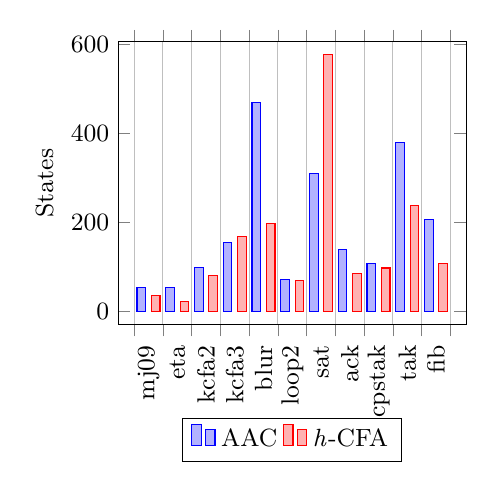
\begin{tikzpicture}
  \small
\begin{axis}[
	symbolic x coords={mj09,eta,kcfa2,kcfa3,blur,loop2,sat,ack,cpstak,tak,fib,empty},
  xtick=data,
	ylabel=States,
	enlargelimits=0.05,
	legend style={at={(0.5,-0.33)},
	anchor=north,legend columns=-1},
	ybar interval=0.6,
  x tick label style={rotate=90},
]
\addplot
	coordinates {(mj09,54) (eta,55)
		 (kcfa2,100) (kcfa3,155) (blur,469) (loop2,72) (sat, 311)
     (ack, 139) (cpstak, 109) (tak,379) (fib,206) (empty,0)};
\addplot
coordinates {(mj09,37) (eta,22)
   (kcfa2,81) (kcfa3,168) (blur,197) (loop2,71) (sat, 577)
   (ack, 86) (cpstak,98) (tak,239) (fib,108) (empty,0)};
\legend{AAC,\textit{h}-CFA}
\end{axis}
\end{tikzpicture}
\caption{monovariant analysis comparison}
\label{0-benchmark}
\endminipage\hfill
\minipage{0.48\textwidth}
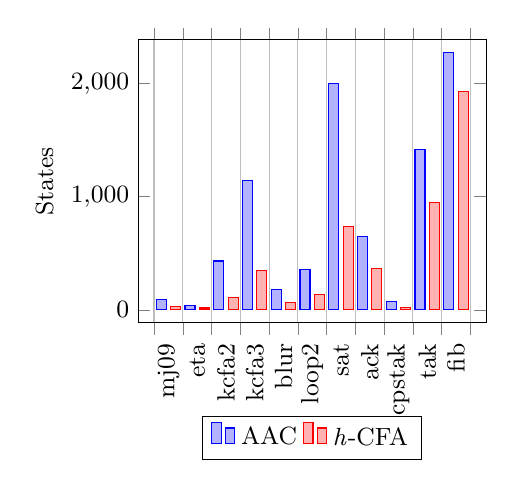
\begin{tikzpicture}
  \small
\begin{axis}[
	symbolic x coords={mj09,eta,kcfa2,kcfa3,blur,loop2,sat,ack,cpstak,tak,fib,empty},
  xtick=data,
	ylabel=States,
	enlargelimits=0.05,
	legend style={at={(0.5,-0.33)},
	anchor=north,legend columns=-1},
	ybar interval=0.7,
  x tick label style={rotate=90},
]
\addplot
	coordinates {(mj09,94) (eta,39)
		 (kcfa2,432) (kcfa3,1145) (blur,183) (loop2,354) (sat, 1999)
     (ack, 645) (cpstak, 73) (tak, 1420) (fib,2273) (empty,0)};
\addplot
coordinates {(mj09,28) (eta,16)
   (kcfa2,110) (kcfa3,348) (blur,63) (loop2,139) (sat, 734)
   (ack, 363) (cpstak, 18) (tak, 945) (fib,1928) (empty,0)};
\legend{AAC,\textit{h}-CFA}
\end{axis}
\end{tikzpicture}
\caption{1-call-site sensitive analysis comparison}
\label{1-benchmark}
\endminipage\hfill
\end{figure}
To illustrate the call/return matching strength of P4F, PDCFA, PDCFA with abstract Garbage Collection (GC), and \textit{h}-CFA, we have
implemented them for Scheme language. We ran the four algorithms on a small program that is similar to the program shown in Figure~\ref{fig:anf-fib}.
The resulting state-transition graphs are shown in Figure~\ref{fig:state-graphs}.

\iffalse
\begin{figure}
  \small
  \lstset{language=Lisp, keywords={define}}
  \begin{lstlisting}
  (define (fib n)
    (if (< n 3)
        1
        (+ (fib (- n 1)) (fib (- n 2)))))

  (define a (fib 10))
  (define b (fib 20))
  (define c (fib 100))
  \end{lstlisting}
\caption{
This example calls Fibonacci function three times
and it is used to compare the strength of call/return matching of four pushdown CFA algorithms.
}
\label{fig:fib}
\end{figure}
\fi

\begin{figure}
\begin{center}
\begin{tabular}{ccc}
%\raisebox{1ex-\height}{
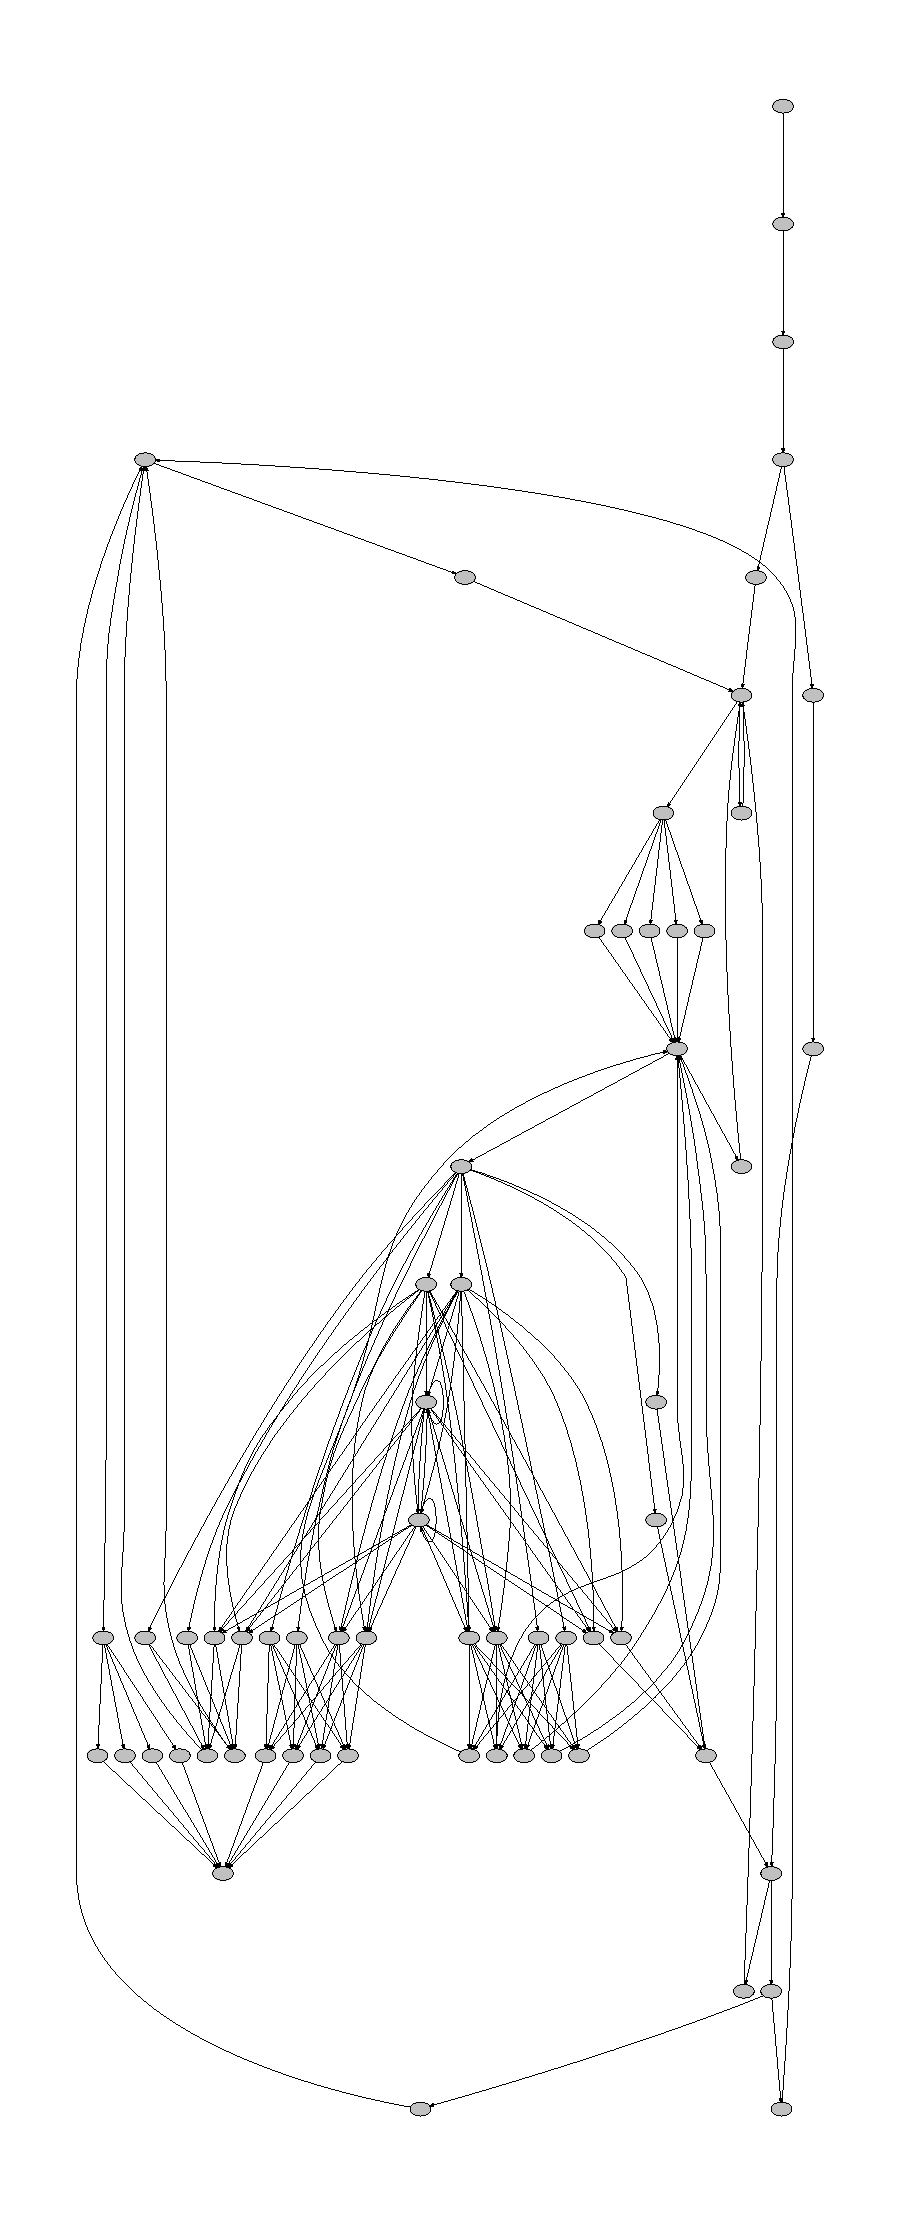
\includegraphics[height=2.5in]{1p4f.pdf}
%}
&
%\raisebox{1ex-\height}{
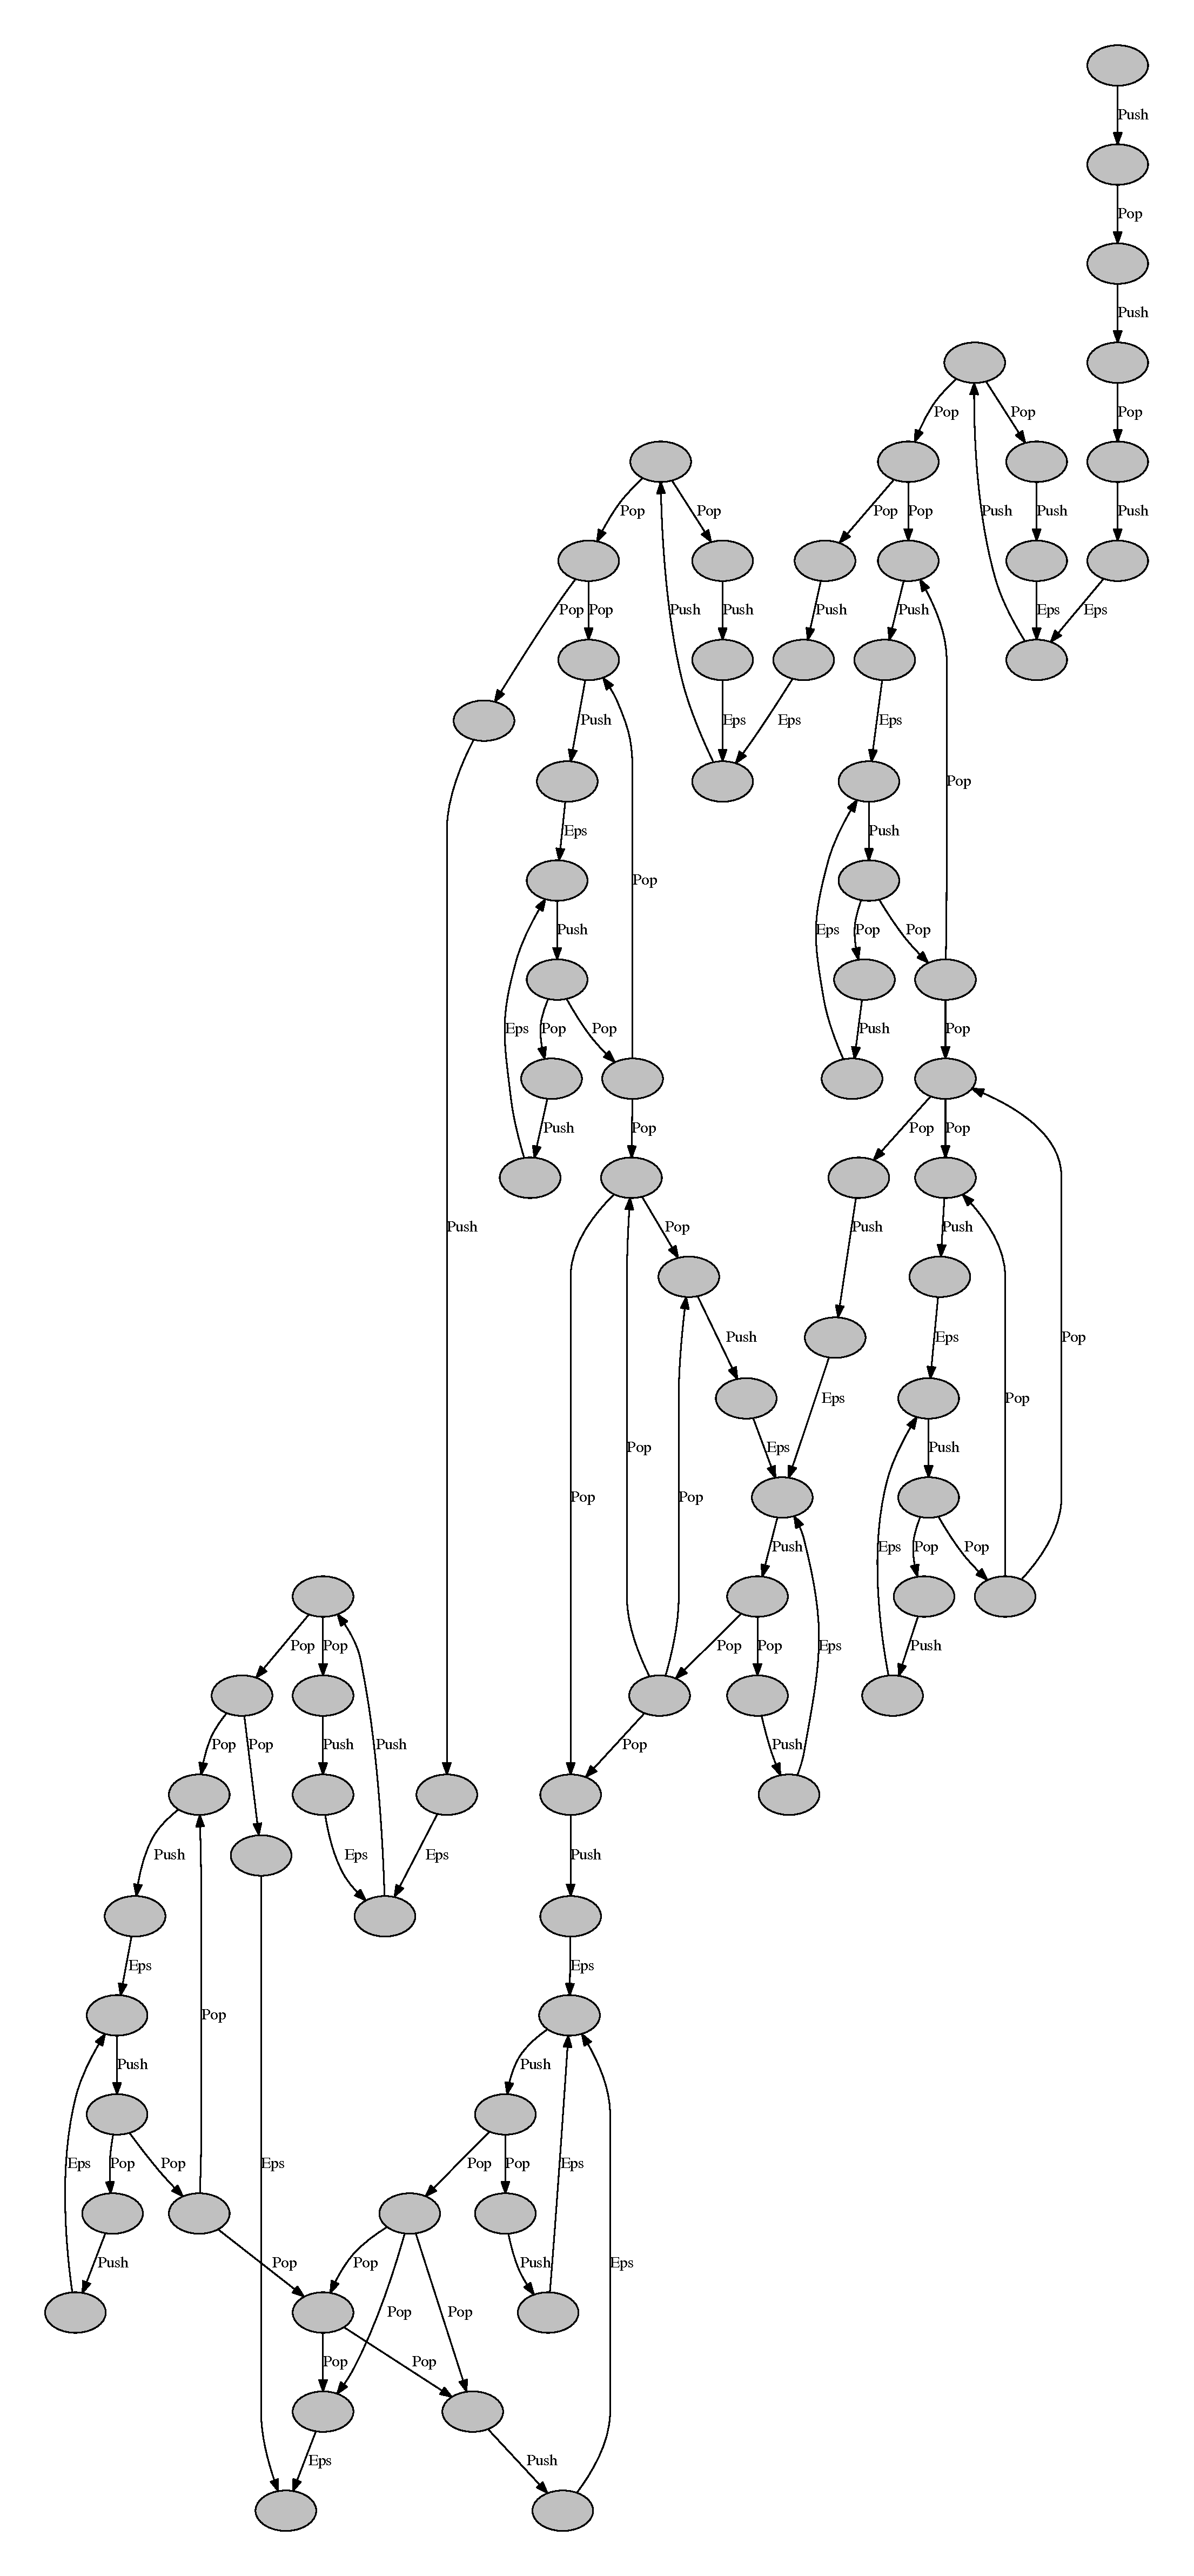
\includegraphics[height=2.5in]{pdcfaWOgc.pdf}
%}
\\
(a) P4F with 1-CFA
&
(b) PDCFA
\\
%\raisebox{1ex-\height}{
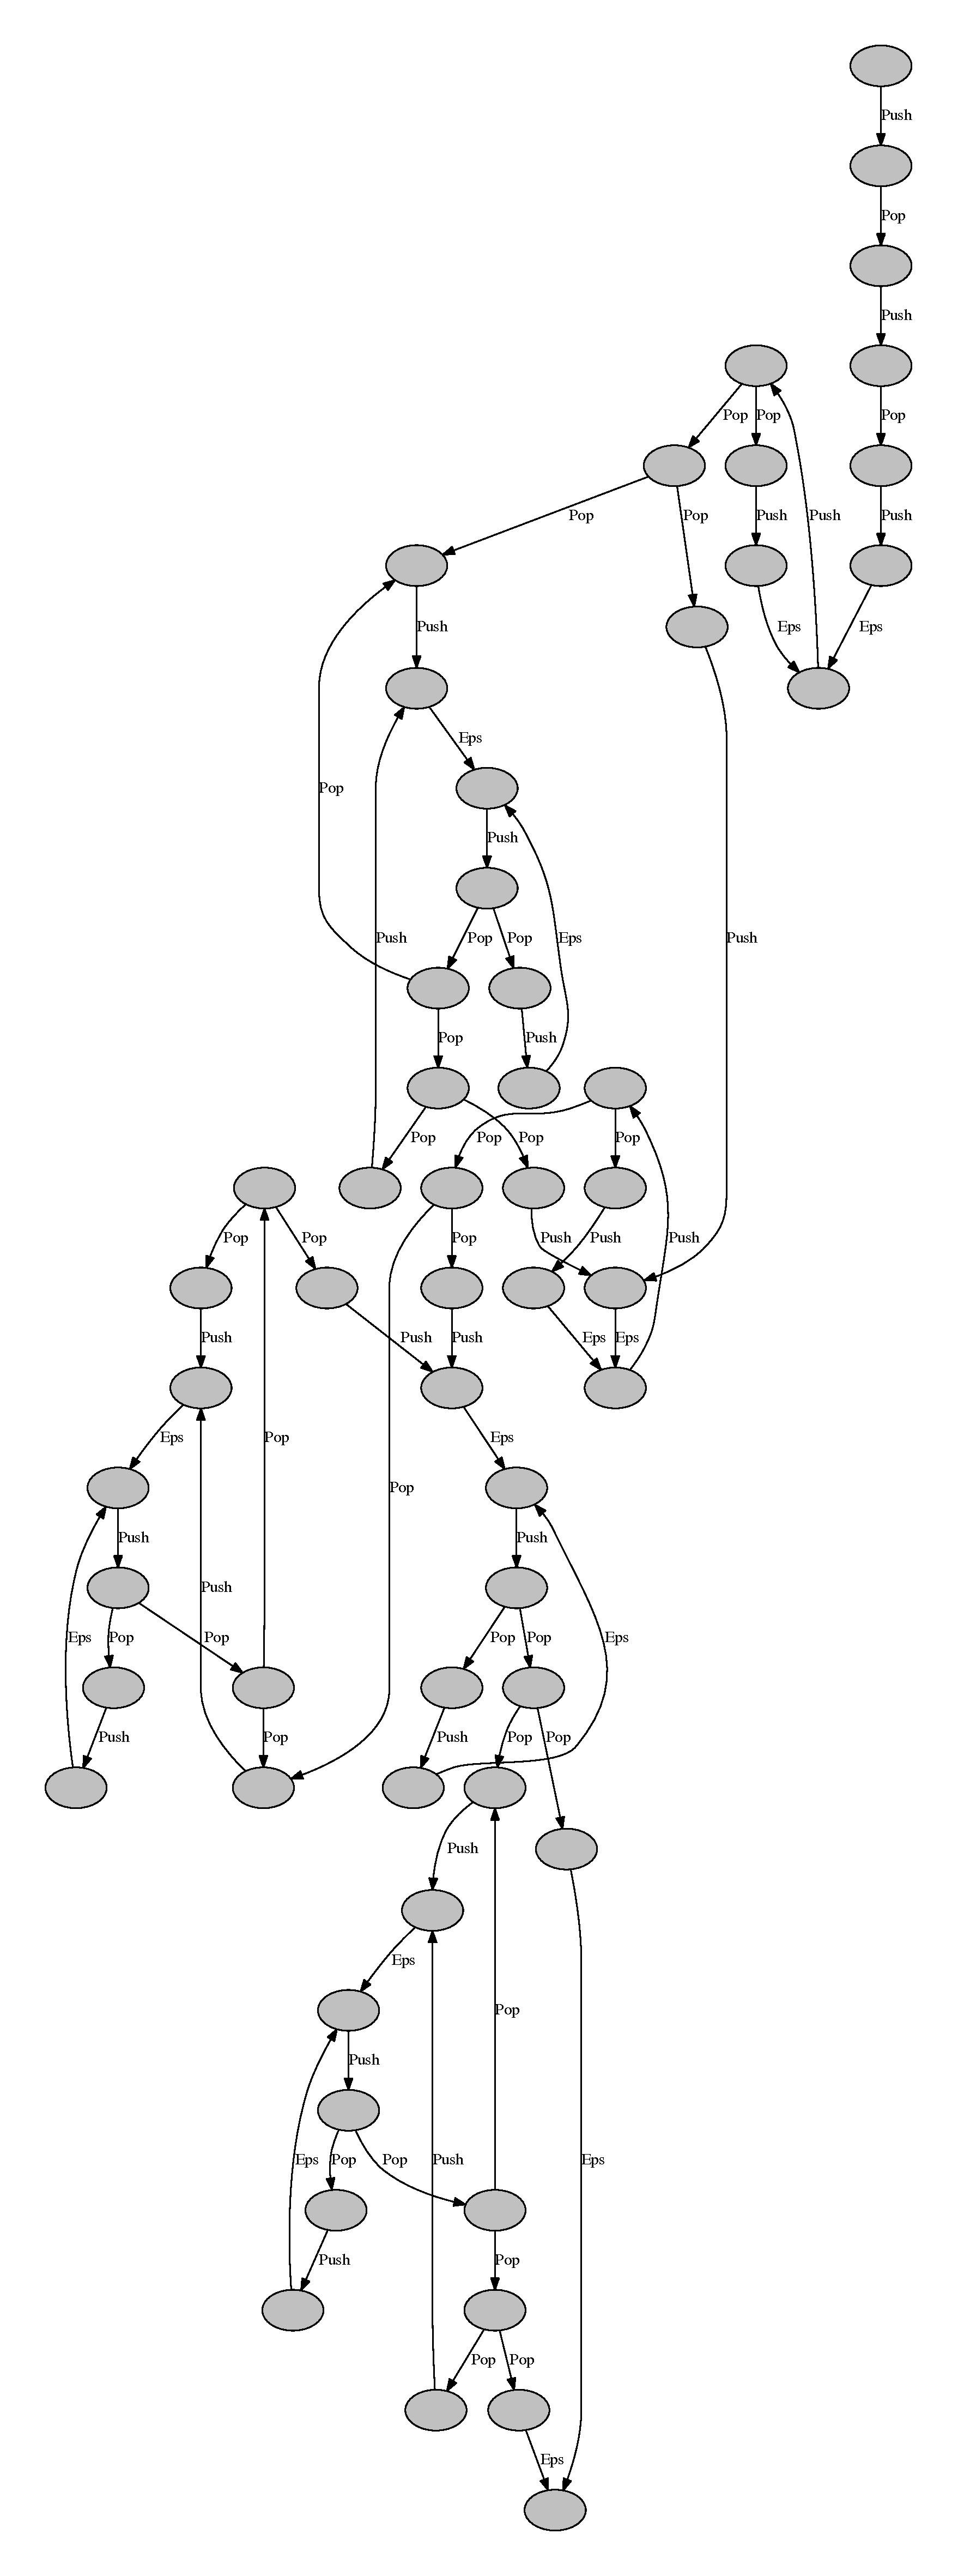
\includegraphics[height=2.5in]{pdcfa.pdf}
%}
&
%\raisebox{1ex-\height}{
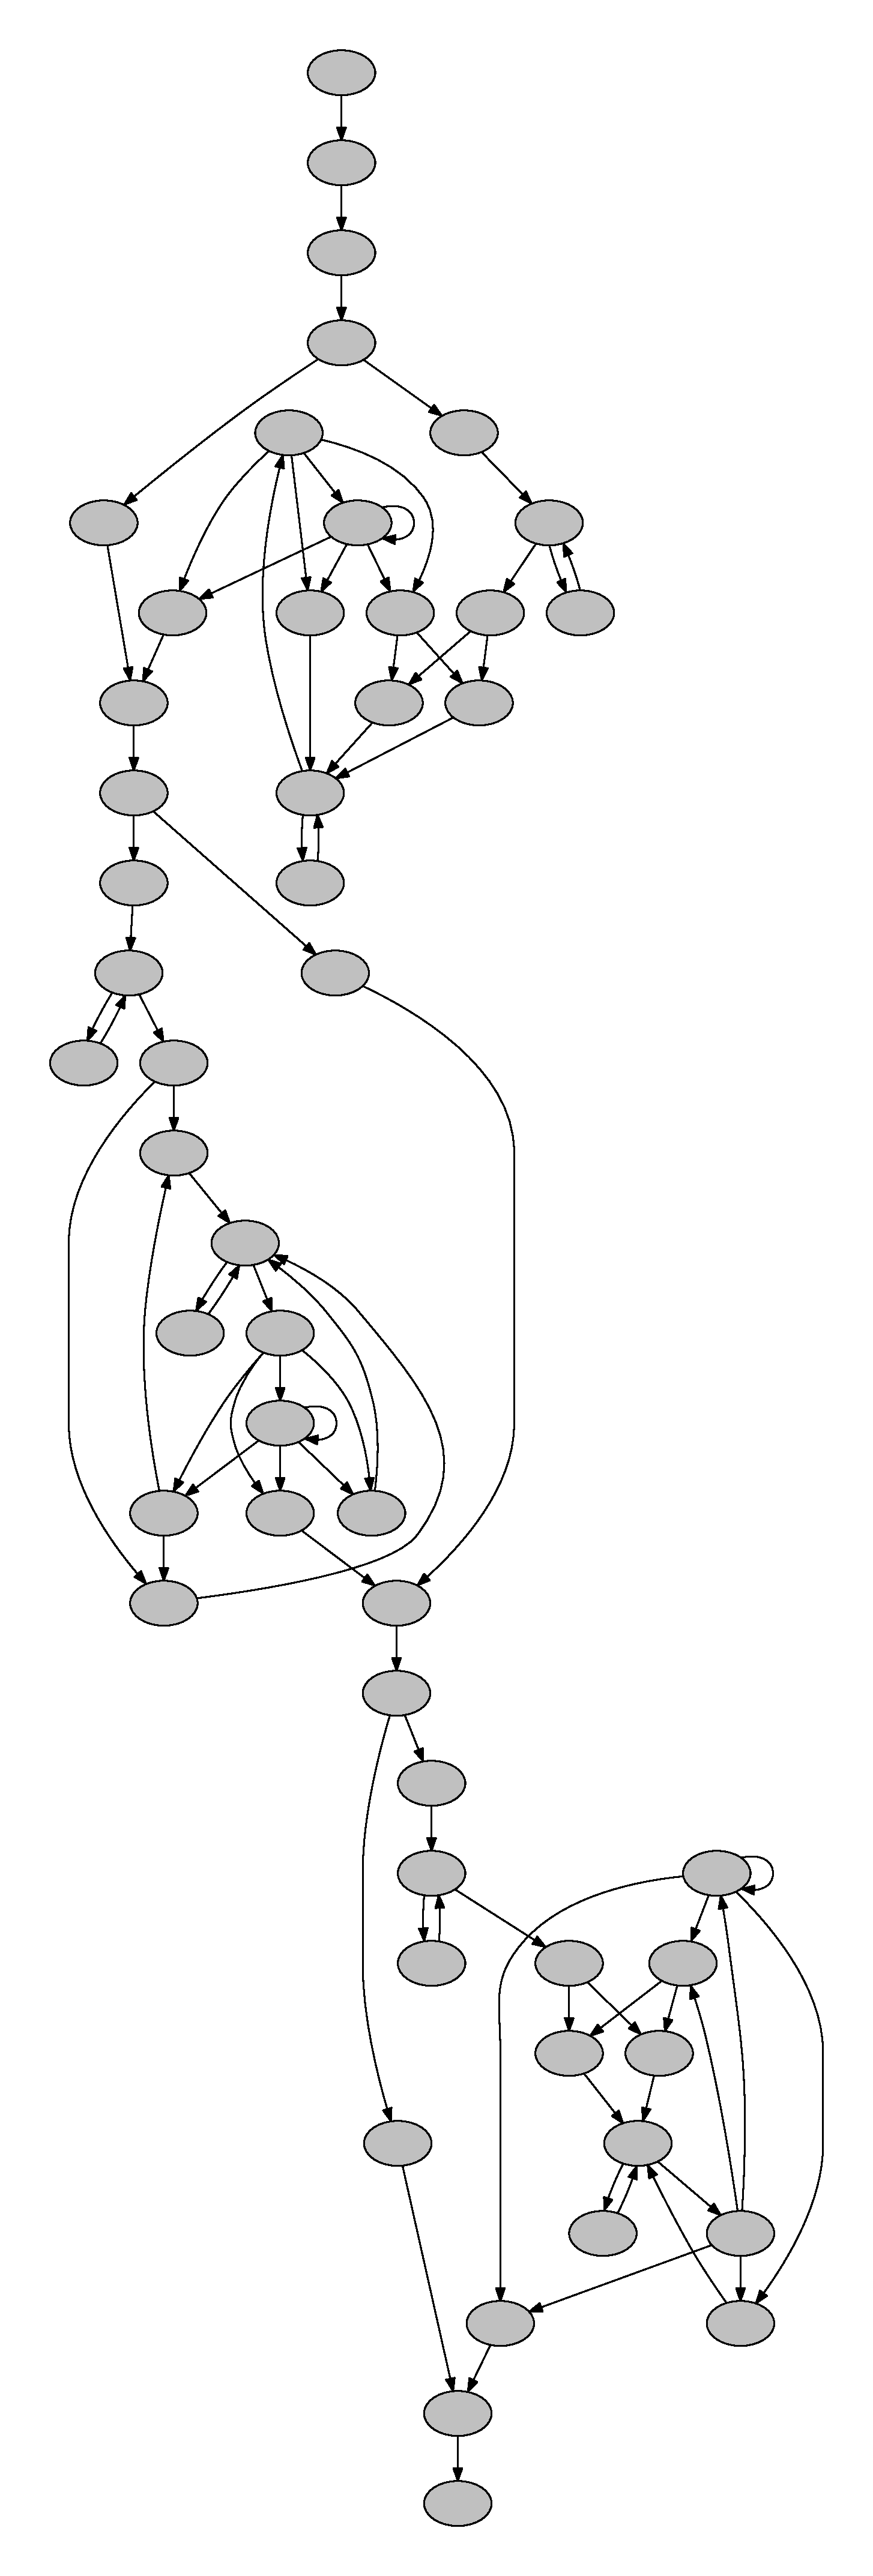
\includegraphics[height=2.5in]{hcfa.pdf}
%}
\\
(c) PDCFA with \\Abstract Garbage Collection
&
(d) \textit{h}-CFA
\end{tabular}
\end{center}
\caption[State transition graphs]{
State transition graphs of: (1) P4F (pushdown CFA for free) with 1-CFA\@;
(2) PDCFA (pushdown CFA); (3) PDCFA with abstract GC\@; (4) \textit{h}-CFA\@.
(2--4) are run with 0-CFA\@.
}
\label{fig:state-graphs}
\end{figure}
As the \textit{h}-CFA graph shows, there are three similar subgraphs in the state transition process, which obviously illustrates
no call/return flow merged in \textit{h}-CFA due to three subgraphs connected by single transition edges.
PDCFA graph also illustrates the similar pattern.
To compare, P4F that just supplies limited call/return matching merges too many control flows in this recursive program.


\iffalse
\section{Defect of \textit{h}-CFA}
\label{sub:Defect of h-CFA}
Although \textit{h}-CFA provides precise call/return flows to monovariance and polyvariance both without extra effort, it just holds on ANF programs. Next section, we will show that certain situations and analysis strategies limit us not being able to compile input programs to ANF before analysis.
Meanwhile, during exploring \textit{h}-CFA, we become clear with why original \textit{k}-CFA cannot perfect match infinite call/return flows. According to this discovery, we develop another pushdown analysis technique that is friendly for direct AST and on longer requires the execution history.
\fi
\chapter{Design of JsCFA}
\label{sec:JsCFA}
JavaScript has become a ubiquitous computing environment in browsers, severs, desktops, even mobile devices. Developers are attracted by its effective and convenient features, such as duck typing, first-class functions, and runtime changeable objects, etc. However, these powerful characters also induce large scale software written in JavaScript to be increasingly unreliable.
In traditional software engineering area, static analysis have become an effective technology to help human to detect deep semantic errors and defects, but the state-of-art in JavaScript static analysis is still not compared with static languages such as C/C++ and Java.

One of the most critical reasons that causes the lag is that JavaScript is a higher-order programming language that treats functions as first-class values. First-class functions can be referred by variables, passed in function arguments, and emitted as return values of other  functions.
In static analysis for higher-order programming languages, control flow analysis often play a significant role because usually we cannot determine which functions are exactly called in a specific call site.
Simultaneously, JavaScript heavily relies on first-class functions to implement certain high-level semantics, such as methods, block scoping, and module import/export, etc.
Consequently, we developed JsCFA, an abstract interpreter for a subset of JavaScript (ECMAScript 3) based on \textit{h}-CFA computes more precise control flow analysis.
Although JsCFA works out almost monovariant, context-insensitive analysis results, AAM allows users to obtain context-sensitivity easily.
Thus we also implemented context-sensitive analysis for certain necessary situations.

This section describes essential pieces of JsCFA designing, including abstract syntax, abstract semantic rules, context-sensitivity, analysis improvement, and usage of \textit{h}-CFA\@.

\section{Syntax Interface}
\label{sub:Syntax}

In JsCFA, we convert JavaScript standard semantics to an unbounded stack small-step abstract machine in CESK style.
The CESK machine operates over direct JavaScript abstract syntax tree (AST) yielded from the parser.
 The abstract syntax tree interface is given in Figure~\ref{fig:js-stmt} and Figure~\ref{fig:js-expr} in Scala code.
Most of the data structures are separated to two categories that inherit from abstract class \verb|Statement| and \verb|Expression| respectively.
JsCFA distinguishes \emph{left values} from \emph{right values} at the syntactical level that simplifies the implementation of CESK machine, so expressions eventually reduced to left values are subclasses of \verb|LValue|.
Trait \verb|AbstractSyntaxTree| defines field \verb|id| to encode the statically and uniquely syntactic label for each AST node. Meanwhile, it decelerates and implements method \verb|generateFrom| that spreads the statically syntactic information from AST nodes to local continuations and values.
The top level of a program is a sequence of statements warped in \verb|Script|.

\begin{figure}
%\small
\lstset{language=Scala,
frame=single,
breaklines=true,
postbreak=\raisebox{0ex}[0ex][0ex]{\ensuremath{\color{red}\hookrightarrow\space}}}
\begin{lstlisting}
  sealed abstract class Statement extends AbstractSyntaxTree

  case class Script(stmts: List[Statement]) extends  Statement
  case class BlockStmt(stmts: List[Statement]) extends Statement
  case class VarDeclListStmt(decls: List[Statement]) extends Statement
  case class EmptyStmt() extends Statement
  case class ExprStmt(expr: Expression) extends Statement()
  case class VarDeclStmt(name: IntroduceVar, expr: Expression) extends Statement
  case class FunctionDecl(name: IntroduceVar, fun: Expression) extends Statement
  case class ReturnStmt(expr: Expression) extends Statement
  case class IfStmt(cond: Expression, thenPart: Statement, elsePart: Statement) extends Statement
  case class SwitchStmt(cond: Expression, cases: List[CaseStmt], defaultCase: Option[CaseStmt]) extends Statement
  case class CaseStmt(expr: Expression, body: Statement) extends Statement
  case class ContinueStmt(continueLabel: String) extends Statement
  case class DoWhileStmt(cond: Expression, body: Statement) extends Statement
  case class WhileStmt(cond: Expression, body: Statement) extends Statement
  case class ForStmt(init: ForInit, cond: Option[Expression], increment: Option[Expression], body: Statement) extends Statement
  case class ForInStmt(init: ForInInit, expr: Expression, body: Statement) extends Statement

\end{lstlisting}
\caption{Abstract syntax tree data types of statements}
\label{fig:js-stmt}
\end{figure}

\begin{figure}
%\small
\lstset{language=Scala,
frame=single,
breaklines=true,
postbreak=\raisebox{0ex}[0ex][0ex]{\ensuremath{\color{red}\hookrightarrow\space}}}
\begin{lstlisting}
  sealed abstract class Expression extends AbstractSyntaxTree

  case class EmptyExpr() extends Expression
  case class FunctionExpr(name: Option[IntroduceVar], ps: List[IntroduceVar], body: Statement) extends Expression with ObjectGeneratePoint
  case class VarRef(name: String) extends Expression with VariableAccess
  case class ThisRef() extends Expression
  case class DotRef(obj: Expression, prop: String) extends Expression
  case class BracketRef(obj: Expression, prop: Expression) extends Expression
  case class MethodCall(receiver: Expression, method: Expression, args: List[Expression]) extends Expression
  case class FuncCall(func: Expression, args: List[Expression]) extends Expression
  case class NewCall(constructor: Expression, args: List[Expression]) extends Expression with ObjectGeneratePoint
  case class AssignExpr(op: AssignOp, lv: LValue, expr: Expression) extends Expression
  case class NullLit() extends Expression
  case class BoolLit(value: Boolean) extends Expression
  case class NumberLit(value: Double) extends Expression
  case class StringLit(value: String) extends Expression
  case class RegExp(regexp: String, global: Boolean, case_insensitive: Boolean) extends Expression with ObjectGeneratePoint
  case class ObjectLit(obj: List[ObjectPair]) extends Expression with ObjectGeneratePoint
  case class ArrayLit(vs: List[Expression]) extends Expression with ObjectGeneratePoint
  case class UnaryAssignExpr(op: UnaryAssignOp, lv: LValue) extends Expression
  case class PrefixExpr(op: PrefixOp, expr: Expression) extends Expression
  case class InfixExpr(op: InfixOp, expr1: Expression, expr2: Expression) extends Expression
  case class CondExpr(cond: Expression, thenPart: Expression, elsePart: Expression) extends Expression
  case class ListExpr(exprs: List[Expression]) extends Expression

  sealed abstract class LValue extends AbstractSyntaxTree

  case class LVarRef(name: String) extends LValue with VariableAccess
  case class LDot(obj: Expression, field: String) extends LValue
  case class LBracket(obj: Expression, prop: Expression) extends LValue
\end{lstlisting}
\caption{Abstract syntax tree data types of expressions}
\label{fig:js-expr}
\end{figure}

\section{Transition Rules}
\label{sub:Transition}

The core data structure of the AAM of JsCFA is class \verb|State| (corresponding to $\tilde{\varsigma}$), which has six components \verb|e| (control string), \verb|env| (environment), \verb|localStack| (intra-procedural continuation stack), \verb|a| (inter-procedural continuation address, or called stack frame pointer), \verb|store| (value store), and \verb|stack| (continuation store). Among them, ``store'' and ``stack'' are packed into the \verb|memory| object that encapsulates certain methods to manipulate the value and continuation store.

\lstset{language=Scala, mathescape}
\begin{lstlisting}
  case class State(e: AbstractSyntaxTree,
                   env: Environment,
                   localStack: LocalStack,
                   a: StackAddress,
                   memory: Memory)

  case class Memory(store: mutable.Map[JSReference, Set[JSValue]],
                    stack: mutable.Map[StackAddress, Set[Frame]]) {
    $\dots$
  }
\end{lstlisting}

The above definition shows two differences from the original AAM and \textit{h}-CFA\@. Class \verb|State| does not contain ``History'' field because we implement \textit{h}-CFA indirectly for JsCFA, and this modification will be discussed in Section~\ref{subs:stack-gc}.
Meanwhile, there is an extra fild \verb|localStack| playing the role of intra-procedural continuation stack, but AAM and \textit{h}-CFA are not. In \textit{h}-CFA, before analysis, ANF transformation already flats all intra-procedural control flows to let-binding, so it just requires to tackle inter-procedural continuations in stores. Besides, original AAM saves all of the continuations (inter and intra-procedural) into continuation stores, but actually only inter-procedural control flows have to be retrieved nondeterministically and intra-procedural continuations are always deterministic.
Consequently, we partition continuations in two places that make semantics clearer and performance better.

JsCFA distinguishes three types of transition states: evaluation, continuation, and application.

\textbf{Evaluation transition} rules accept a state and match its control string component to generate successors. Evaluation transitions firstly search values and reducible expressions/statements (we refer states carry reducible expressions/statements to complete states in JsCFA) in the control strings.
If the control string is a value (instance of class \verb|JSValue|), analysis would be dispatched to a continuation transition that depends upon  the following control flow step retrieved from the top of local stack. Then the continuation transition determines how to use the value.
If the current state is a complete state that its every recursive component is already computed to a value, the abstract machine transits to application to execute main semantics of the AST node.
Eventually, when the control string is neither value nor reducible expression/statement, the machine generates the new continuation according to semantics of standard JavaScript.
Then the new continuation is pushed on the local stack and the machine proceeds to evaluate the program point whose computing result is required firstly.
Finally, there is a special circumstance in dispatching to continuation transitions. If the local stack is empty (no valid \verb|cont| in Figure~\ref{fig:eval}), that means there is no ``next step'' in current execution context and the function does not have a return statement along the current execution path.
Therefore, we have to implement ``return'' semantics at this point too while the executing function returns \verb|undefined| to its return point restored from stack frames.

\begin{figure}
%\small
\lstset{language=Scala, mathescape}
\begin{lstlisting}
  def transitEvaluation(state: State): Set[State] = state match {
    case completeState if isComplete(completeState) =>
        transitApplication(state)
        //dispatch to application transition
    case State(v, env, localStack, a, memory) if isJSValue(v) =>
        if (localStack.nonEmpty) {
          val cont = topOfLocalStack(localStack)
          val newStack = popLocalStack(localStack)
          transitContinuation(cont, v, env, newStack, a, memory)
          //dispatch to continuation transition
        } else {
          $\dots$ \\return
        }

    //statements
    case State(Script(Nil), env, localStack, a, memory) =>
        Set(State(Halt, env, localStack, a, memory))
    case State(Script(stmt :: ss), env, localStack, a, memory) =>
        val k = KScript(ss)
        k.generateFrom(state.e)
        val newStack = pushLocalStack(localStack, k)
        Set(State(stmt, env, newStack, a, memory))

    case State(ReturnStmt(e), env, localStack, a, memory) =>
        val k = KReturn()
        k.generateFrom(state.e)
        val newStack = pushLocalStack(localStack, k)
        Set(State(e, env, newStack, a, memory))

    case State(IfStmt(cond, t, e), env, localStack, a, memory) =>
        val k = KIfCond(t, e)
        k.generateFrom(state.e)
        val newStack = pushLocalStack(localStack, k)
        Set(State(cond, env, newStack, a, memory))
    $\dots$

    //expressions
    case State(FuncCall(func, args), env, localStack, a, memory) =>
        val k = KFuncCallF(args)
        k.generateFrom(state.e)
        val newStack = pushLocalStack(localStack, k)
        Set(State(func, env, newStack, a, memory))

    case State(AssignExpr(op, lv, expr), env, localStack, a, memory) =>
        val k = KAssignR(op, lv)
        k.generateFrom(state.e)
        val newStack = pushLocalStack(localStack, k)
        Set(State(expr, env, newStack, a, memory))

    case State(InfixExpr(op, e1, e2), env, localStack, a, memory) =>
        val k = KInfixL(op, e2)
        k.generateFrom(state.e)
        val newStack = pushLocalStack(localStack, k)
        Set(State(e1, env, newStack, a, memory))
    $\dots$
  }
\end{lstlisting}
\caption{Parts of Evaluation Transition Rules}
\label{fig:eval}
\end{figure}

\textbf{Continuation transitions} work on the six components that state objects have and an extra \emph{next continuation} (referred to as \verb|cont| in Figure~\ref{fig:cont-stmt} and Figure~\ref{fig:cont-expr}).
Control strings in these transition states are alway values, so abstract machines dispatch transitions via matching \verb|cont| and plug the value into a new continuation.
If the new continuation object is a reducible expression/statement, the next machine states will move to application transitions.
Under this situation, the new continuation object is a \emph{complete} expression/statement that will be placed on control string position of next state.
Otherwise, the new continuation that contains the value of control string is pushed into the local stack.
Then, the following computing will be dispatched by next evaluation states.

\begin{figure}
\lstset{language=Scala, mathescape}
\begin{lstlisting}
  def transitContinuation(cont: Continuation,
                          value: JSValue,
                          env: Environment,
                          localStack: LocalStack,
                          a: StackAddress,
                          memory: Memory): Set[State] = cont match {
    case KScript(Nil) =>
        Set(State(Halt, env, localStack, a, memory))
    case KScript(s :: ss) =>
        val k = KScript(ss)
        k.generateFrom(cont)
        val newStack = pushLocalStack(localStack, k)
        Set(State(s, env, newStack, a, memory))

    case KReturn() =>
        val k = KReturnComplete(value)
        k.generateFrom(cont)
        Set(State(k, env, localStack, a, memory))

    case KIfCond(t, e) =>
        val k = KIfComplete(value, t, e)
        k.generateFrom(cont)
        Set(State(k, env, localStack, a, memory))
    $\dots$
\end{lstlisting}
\caption{Parts of Continuation Transition Rules for Statements}
\label{fig:cont-stmt}
\end{figure}

\begin{figure}
\lstset{language=Scala, mathescape}
\begin{lstlisting}
    case KFuncCallF(Nil) =>
        val k = KFuncCallA(value, Nil, Nil)
        k.generateFrom(cont)
        val newStack = pushLocalStack(localStack, k)
        Set(State(cachedUndefined, env, newStack, a, memory))

    case KFuncCallF(arg :: args) =>
        val k = KFuncCallA(value, Nil, args)
        k.generateFrom(cont)
        val newStack = pushLocalStack(localStack, k)
        Set(State(arg, env, newStack, a, memory))

    case KFuncCallA(func, before, Nil) =>
        val k = KFuncCallComplete(func, before ++ List(value))
        k.generateFrom(cont)
        Set(State(k, env, localStack, a, memory))

    case KFuncCallA(func, before, arg :: args) =>
        val k = KFuncCallA(func, before ++ List(value), args)
        k.generateFrom(cont)
        val newStack = pushLocalStack(localStack, k)
        Set(State(arg, env, newStack, a, memory))

    case KAssignR(op, lv) =>
        val k = KAssignL(op, value)
        k.generateFrom(cont)
        val newStack = pushLocalStack(localStack, k)
        Set(State(lv, env, newStack, a, memory))

    case KAssignL(op, rv) =>
        val k = KAssignExprComplete(op, value, rv)
        k.generateFrom(cont)
        Set(State(k, env, localStack, a, memory))

    case KInfixL(op, e2) =>
        val k = KInfixR(op, value)
        k.generateFrom(cont)
        val newStack = pushLocalStack(localStack, k)
        Set(State(e2, env, newStack, a, memory))

    case KInfixR(op, e1) =>
        val k = KInfixExprComplete(op, e1, value)
        k.generateFrom(cont)
        Set(State(k, env, localStack, a, memory))
    $\dots$
  }
\end{lstlisting}
\caption{Parts of Continuation Transition Rules for Expressions}
\label{fig:cont-expr}
\end{figure}

\textbf{Application transitions} just accept complete states to generate subsequent states. Function \verb|isComplete| exams whether the passed-in state is complete by matching its control string.
Complete control strings represent the expressions/statements always reducible.
They are either AST nodes direct from the parser or continuation objects generated by continuation transitions. These application transitions described in Figure~\ref{fig:app-stmt} and Figure~\ref{fig:app-expr} implement all the reduction rules of JavaScript.

\begin{figure}
\lstset{language=Scala, mathescape}
\begin{lstlisting}
def transitApplication(state: State): Set[State] = state match {
  case State(KReturnComplete(v), env, localStack, a, memory) =>
      val newMemory = memory.copy(state)
      for {
        Frame(returnPoint, oldStack, savedEnv, newGlobalAddress)
            <- newMemory.getFrames(a) //get the stack frame
      } yield {
        if(oldStack.isEmpty ||
          !oldStack.head.isInstanceOf[KUseValue]) {
          //if current function called by "new", return "this" object
          for(vs <- newMemory.getValues(v)) {
            newMemory.putValue(returnPoint, vs)
          }
        }
        State(returnPoint, savedEnv,
              oldStack, newGlobalAddress, newMemory)
      }

  case State(KIfComplete(cond, t, e), env, localStack, a, memory) =>
      for {
        obj <- memory.getValues(cond)
        boolValue = ToBoolean(obj)
        res <- boolValue match {
          case JSBoolean(ConstantBoolean(true)) =>
              Set(State(t, env, localStack, a, memory))
          case JSBoolean(ConstantBoolean(false)) =>
              Set(State(e, env, localStack, a, memory))
          case JSBoolean(VariableBoolean) =>
              Set(State(t, env, localStack, a, memory),
              State(e, env, localStack, a, memory))
        }
      } yield res
  $\dots$

\end{lstlisting}
\caption{Parts of Application Transition Rules for Statements}
\label{fig:app-stmt}
\end{figure}

\begin{figure}
\lstset{language=Scala, mathescape}
\begin{lstlisting}
  case State(VarRef(x), env, localStack, a, memory) =>
      val newMemory = memory.copy(state)
      val xRef = lookup(env, x)
      for(vs <- newMemory.getValues(xRef)){
        newMemory.putValue(JSReference(state.e.id), vs)
      }
      Set(State(JSReference(state.e.id), env, localStack, a, newMemory))

  case State(LVarRef(x), env, localStack, a, memory) =>
      val xRef = lookup(env, x)
      // lvalues are addresses
      Set(State(xRef, env, localStack, a, memory))

  case State(f@FunctionExpr(name, ps, body), env, localStack, a, memory) =>
      val newMemory = memory.copy(state)
      val functionObject = createFunctionObject(f, env, newMemory)
      val value = newMemory.save(functionObject)
      Set(State(value, env, localStack, a, newMemory))

  case State(NumberLit(num), env, localStack, a, memory) =>
      val newMemory = memory.copy(state)
      val number = JSNumber(ConstantNumber(num))
      number.generateFrom(state.e)
      val value = newMemory.save(number)
      Set(State(value, env, localStack, a, newMemory))

  case State(KAssignExprComplete(op, lv, rv), env, localStack, a, memory) =>
      val newMemory = memory.copy(state)
      for(value <- newMemory.getValues(rv)) {
          newMemory.putValue(lv.asInstanceOf[JSReference], value)
      }
      Set(State(rv, env, localStack, a, newMemory))

  case State(KInfixExprComplete(op, rv1, rv2), env, localStack, a, memory) =>
      val newMemory = memory.copy(state)
      for {
          v1 <- newMemory.getValues(rv1)
          v2 <- newMemory.getValues(rv2)
      } yield {
          val res = infixFunc(op, v1, v2, newMemory)
          res.generateFrom(state.e)
          val address = newMemory.save(res)
          State(address, env, localStack, a, newMemory)
      }
  $\dots$
}
\end{lstlisting}
\caption{Parts of Application Transition Rules for Portions of Expressions}
\label{fig:app-expr}
\end{figure}

Once the abstract interpreter of JsCFA launches, the parser reads input program and convert it to an AST warped as a \verb|Script| object at top level.
Then \verb|inject| takes the AST to generate initial machine state that contains all JavaScript built-in variables, objects, and functions into $\widetilde{initEnv}$ and $\widetilde{initMemory}$. Then worklist algorithm starts evaluation transition on the initial state.
\[
inject_{JsCFA} : AbstractSyntaxTree \to State
\]
\[
inject_{JsCFA}(script) = State(script, \widetilde{initEnv}, \varnothing, \widetilde{a_k{}_{init}}, \widetilde{initMemory})
\]

\section{Store and Stack}
\label{sub:Store and Stack}

Class \verb|Memory| packs value store and continuation store in one object and provides four main methods for interacting with abstract machines.
\[
putValue: Memory \times JSReference \times JSValue \to Unit
\]
\[
getValues: Memory \times JSReference \to \mathcal{P}(JSValue)
\]
\[
pushFrame: Memory \times StackAddress \times Frame \to Unit
\]
\[
getFrames: Memory \times StackAddress \to \mathcal{P}(Frame)
\]

Method \verb|putValue| and \verb|pushFrame| imperatively updates value store and continuation store respectively.
They both join the given value/frame to existing elements that already inhabit in the address.

\[
m.putValue(a, v) = this.store[a] := this.store(a) \cup \{v\}
\]
\[
m.pushFrame(a, f) = this.stack[a] := this.stack(a) \cup \{f\}
\]
Meanwhile, \verb|getValues| and \verb|getFrames| retrieves values and stack frames nondeterministically.
\[
m.getValues(a) = this.store(a)
\]
\[
m.getFrames(a) = this.stack(a)
\]

\section{Functions, Methods, and Constructors}
\label{sub:Functions, Methods, and Constructors}

The semantics of function invocation in JavaScript is more complex than other programming languages.
There are three patterns of invocations, function call, method call, and new call.

Application transition rule of function call is shown in Figure~\ref{fig:app-call}, which extracts called functions (closures in function objects) and arguments by \verb|getValues|, and extends the closure environment with these arguments. Then, \verb|this| is also regarded as an implicit paramter and we map \verb|this| to the address of global object (\verb|window| in browser environment and \verb|global| in ``node.js''). Next, we save the current computing context (return point, local stack, evaluation environment, and stack pointer) to a frame and push it on the stack (continuation store).
The address of top of stack is generated by function \verb|allocStackAddress|, which implements the call/return strategy of JsCFA and we will describe it in Section~\ref{subs:stack-gc}. Finally, the abstract interpreter is going to evaluate the function bodies with extended environments and an empty local stack.

\begin{figure}
  \lstset{language=Scala}
  \begin{lstlisting}
case State(KFuncCallComplete(funcRef, args), env, localStack, a, memory) =>
    val newMemory = memory.copy(state)
    for {
        f <- newMemory.getValues(funcRef) //get function objects
        if isCallable(f)
        JSClosure(func@FunctionExpr(name, ps, funcBody), savedEnv) =
            f.asInstanceOf[JSObject].code
            //get closures from the function object
    } yield {
        val psAddress = ps.map(alloc(_))
        //allocate addresses for formal parameters
        val thisAddress = biGlobalObjectRef
        // address of global object
        var newEnvPart =
          ("this" -> thisAddress) :: ps.map(x => x.str).zip(psAddress)
          //extend environment with "this" and other parameters
        name match {
          case Some(x) => newEnvPart = (x.str -> alloc(x)) :: newEnvPart
            ////extend environment with the function name
          case None =>
        }
        val newEnv = savedEnv ++ Map(newEnvPart: _*)

        for(p <- psAddress.zip(args)) {
          for(vs <- newMemory.getValues(p._2)) {
            newMemory.putValue(p._1, vs)
              //pass actual parameters to formal parameters
          }
        }

        val nextAddress = allocStackAddress(state, funcBody, newEnv)
          //allocate the stack frame
        newMemory.pushFrame(nextAddress,
                            Frame(alloc(state.e), localStack, env, a))
        State(funcBody, newEnv, emptyLocalStack, nextAddress, newMemory)
    }

  \end{lstlisting}
  \caption{Application Transition Rule for Global Function Calls}
\label{fig:app-call}
\end{figure}

Because JavaScript is a prototype-based object-oriented language, it uses first-class functions to implement methods and constructors of objects.
Therefore, the only difference between function calls and method calls is that method invocations extract function objects from receivers and explicitly bring \verb|this| arguments, so we need to set \verb|this| to ``receivers'' in method environments.
New call (functions called as constructors) is another function invocation form in JavaScript, which generates a new and empty object at the ``new call site'', and passes the object as \verb|this| parameter. Finally abstract interpreters return the generated object as computing result of the new call.
In JsCFA, we implement the ``return the generated object'' by a trick, which puts an extra local continuation object \verb|KUseValue(obj)| into the new \verb|localStack|.
\verb|KUseValue(obj)| represents a low-level instruction that indicates that abstract interpreter should throw away functions' original return values and use the specific object \verb|obj| that is created at the ``new call site'' to replace.

\section{Configureable Context-Sensitivity and Adaptive Object-Sensitivity}
\label{sub:Configureable}
Context sensitivity is an effective approach to impact precision and performance of static analysis.
Different context choices yield different analysis results and performance.
On the one hand, each kind of context sensitivity strategy (call-site sensitive~\cite{shivers1991control}, argument sensitive~\cite{agesen1995cartesian}, object sensitive~\cite{milanova2005parameterized, smaragdakis2011pick}, field sensitive~\cite{lhotak2003scaling}, etc.) just contributes considerable precision influence on specific analysis problems.
On the other hand, certain contexts can select different precision levels with different performance costs, such as call-site sensitivity in \textit{k}-CFA\@.
One of the most crucial contributions of AAM is that makes context sensitivity configureable.
Contexts of polyvariant values are only determined by $\widetilde{alloc}$ and data type of $\widetilde{Addr}$. %cite
Even we can mix several context sensitivity strategies in one analyzer.
For example, JsCFA usually allocates context insensitive addresses for most values by $\widetilde{alloc_{JsCFA}}$ below.
\[
\widetilde{alloc}_{JsCFA}(expression) = JSReference(expression.id)
\]
Every expression store its computing result (values) in the slot indicated by its static syntactical label (\verb|expression.id|).
However, the context insensitive addresses will dramatically lose precision over dynamic features of JavaScript.
First of all, the object model of JsCFA is almost similar to $\lambda_{JS}$~\cite{guha2010essence}, which regards JavaScript objects as maps.
\[
JSObject : JSString \to JSReference
\]
Keys of objects are strings mapping to addresses that point to actual values in the store.
Additionally, each object contains two special key/value pairs, \verb|"__proto__"| and \verb|"constructor"|, which is used to implement prototype-based inheritance of JavaScript.

Then, consider the following common example code in JavaScript, which dynamically adds fields to objects.
\lstset{mathescape}
\begin{lstlisting}
  obj["p"] = e$^l$ //"p" is not in obj
\end{lstlisting}
In totally monovariant analysis, if several objects flow into \verb|obj| simultaneously or sequently, after the expression executing all of the objects would have a field \verb|"p"| that points to values allocated in \verb|JSReference(l)|.
However, if other expressions reassign the value of field \verb|"p"| for one of these objects, this modification will propagate to each object that flowed into \verb|obj|.

Thus, we apply object sensitive allocation for the dynamic object extension.
\[
\widetilde{alloc}^{o}_{JsCFA}(expression, object) = JSReference(expression.id, object.id)
\]
This object sensitive allocation function separates dynamically added fields to different dimension for each object. Only application transition rules of \verb|LDot| and \verb|LBracket| use $\widetilde{alloc}^{o}_{JsCFA}$ for adding fields, and other situations maintain context insensitive.
Ultimately, JsCFA achieves more precise analysis over dynamic objects, but no heavy overhead imported.

\section{Abstract Garbage Collection as Stack Filtering}
\label{sub:filtering}
In practice, call/return perfect match only working with monovariant analysis is useless.
Please consider the first simple example in Section~\ref{Introduction} again: if our abstract interpreter can match call/return flows perfectly, variable \verb|a| would get value \verb|1| after executing call site 1. Then, when call site 2 invokes function \verb|id| again, the new argument \verb|#t| merges with \verb|1| that was passed into \verb|x| by call site 1.
Then, the merged abstract value \verb|{1, #t}| returns to variable \verb|b|.
Meanwhile, this spurious analysis result will flow into the following interpretation, and accumulated spurious values and flows will dramatically decrease the precision of analysis.
This problem will cause more critical imprecision in higher-order languages, which is referred to as environment problem~\cite{shivers1991control}.
\lstset{
keywords={function, return}}
\begin{lstlisting}
function compose-same(f, x) {
  return f(f(x));
}
\end{lstlisting}
In \verb|compose-same|, local variable \verb|f| is referring to functions and called twice.
In actual runtime, these two call sites always invoke the same function.
However 0-CFA or \textit{k}-CFA without enough context length may compose different closures for these two call sites when \verb|compose-same| is called multiple times and several different functions flow into \verb|f|.
This spurious control flow problem (a.k.a.\ fake rebinding~\cite{vardoulakis2010cfa2}) not only yields bad analysis result, but also increases the running time of the analysis.
Traditional \textit{k}-CFA attempts to resolve this problem via introducing context-sensitive (polyvariant) analysis.
However, polyvariance is not an efficient and powerful solution to this problem.

The essential reason why different actual parameters merge into the same formal parameters is monovariant abstract interpreters breaking the concrete semantics. Concrete interpreters never merge parameters from different call sites because local variables will be deleted when the interpreter exits from the function.
Consequently, CFA2 invents an approach named ``stack filtering'' making it more useful, which just returns \verb|#t| to variable \verb|b|. Stack filtering simulates the semantics of popping call stack frames to remove useless values of local variables. However, there are two limitations that lead stack filtering not being able to port to AAM\@. On the one hand, AAM adopts reference model for all of the values (all things in stores), but CFA2 has stack allocated values. On the other hand, we cannot always pop call stack frames after function returns because Section~\ref{sub:Polyvariant Continuation} mentions that continuation stores may become graphs that contain cycles rather than stacks.

Introspective pushdown control flow analysis~\cite{earl2012introspective} described by Earl, Sergey, Might, and Van Horn integrates abstract garbage collection~\cite{might2006improving} in PDCFA to implement stack filtering. JsCFA also adopts this strategy to improve analysis precision and make call/return match more useful. The semantics of abstract garbage collection is the same with its counterparts in concrete interpreters/runtimes.
We first scan current state to acquire the root set and trace from the root set to reach all the objects' fields and closures' caught variables. Every address reached in the last phase (computing root set and tracing) is recorded in a ``mark set'', and values referred by addresses that do not appear in the mark set are regarded as garbage.

However, the effect of abstract garbage collection is relatively weaked in global store because the values referred by other unexecuted paths have to stay in the store even though current state cannot reach them.
Therefore, Earl et al.\ implemented PDCFA with abstract GC with per-state stores to achieve the whole power of abstract GC\@.
Although AAM with per-state stores theoretically takes exponential complexity, in practice its performance much better than global store without abstract GC\@.
Consequently, we also implement JsCFA with per-state stores. Moreover, there are two techniques to optimize performance of abstract GC with per-state stores. Firstly, JsCFA just copies stores on write because only application states may change the store, so evaluation and continuation states interpreted between two application states share one store.
Secondly, abstract GC running never directly deletes values even if they are detected as garbage. When the abstract interpreter requires a new copied store, we just copy values that are referred by mark set (reached values) to eliminate the overhead of imperative deleting elements in stores.
Class \verb|Memory| provides method \verb|copy| that launches GC and returns a new memory instance only containing reachable elements.
\[
copy: Memory \times State \to Memory
\]
\section{Pushdown CFA without Program Execution History}
\label{sub:pushdown-jscfa}
\textit{h}-CFA is an effective and easily implemented method to acquire call/return perfect match in monovariant analysis on ANF style programs. However, ANF transformation limits precision improvement of highly dynamic language analysis, especially JavaScript.
Although theoretical static analysis techniques already obtain acceptable consequence for higher-order programming languages, it is still not enough for realistic dynamic languages. For example, because JavaScript is a prototype-type based language that has no native ``inheritance'' semantics, programmers usually implement their own ``inherit'' or ``extend'' functions to simulate object-oriented inheritance.
\lstset{mathescape,
keywords={function, for, in, if, return, var}}
\begin{lstlisting}
  function extend(target, source) {
    for(var propName in source) {
      if(source.hasOwnProperty(propName)) {
        target[propName] = source[propName];
      }
    }
    return target;
  }
\end{lstlisting}
The function \verb|extend| accepts two objects as parameters, \verb|target| and \verb|source|.
Then all of the first-level properties of object \verb|source| are copied into \verb|target|. If we apply traditional static analysis (points-to analysis) techniques to programs that densely use this function, the precision would be dramatically decreased.
Consider monovariant analysis on function \verb|extend|, all property names (strings) of \verb|source| flows into \verb|propName| and merges to a ``variable string'' (top value of string in JsCFA), and object \verb|target| also becomes a top value of object that does not contribute any benefit to the following analysis process.
Traditional monovariant analysis does not detect and fulfill the high-level semantics that copy first-level properties form one object to others.
Fortunately, there are already techniques that attempt to boost static analysis results for dynamic languages via recognizing high-level semantics.
Correlation tracking~\cite{sridharan2012correlation}
is one of these techniques that matches \emph{correlated dynamic property access} patterns that are often used to implement \verb|extend|. Then analysis precision achieves enhancement from the high-level perspective that directly ``inherit'' properties from \verb|source|.
Therefore, we have to retain code patterns or conventions of input programs in the intermediate representations (IR) of abstract interpreters.
This is the most significant reason why we adopt direct AST as the IR of JsCFA rather than other low-level forms, such as ANF\@.

However, it would introduce extra effort to record the program execution history if we port \textit{h}-CFA to cooperate with direct AST in JsCFA\@. Consequently, JsCFA adopts \textit{h}-CFA by an indirect approach that can perfect match call/return flows without program execution histories.

\subsection{The Essence of \textit{h}-CFA}
\label{subs:ehcfa}
Before adjusting \textit{h}-CFA for JsCFA, we should discuss the most significant reason why abstract interpreters require program execution history for pushdown CFA\@. Consider the example in Figure~\ref{fig:anf-fib} again: after analyzing \verb|(a (fib 10))|, function \verb|fib| is invoked again and we have to recompute the recursive call site \verb|(fib res2)| in a new analysis environment. At this point, the continuation store $\widetilde{\sigma_k^H}$ looks like below.
\[
\widetilde{a^H_k{}_{11}} = ((fib\ 10), \widehat{fib}, \{fib\})
\]
\[
\widetilde{a^H_k{}_{12}} = ((fib\ res2), \widehat{fib}, \{fib, res1, res2\})
\]
\[
\widetilde{a^H_k{}_{21}} = ((fib\ 20), \widehat{fib}, \{fib, a\})
\]
\[
\widetilde{a^H_k{}_{22}} = ((fib\ res2), \widehat{fib}, \{fib, a, res1, res2\})
\]
\[
\begin{aligned}
\widetilde{\sigma_k^H} = \{ {}& \widetilde{a^H_k{}_{11}} \mapsto \{(a, (let\ (b\ (fib\ 20))\ \dots), \widetilde{env_1}, \{fib\}, \widetilde{a^H_k{}_{init}})\}  {} \\
                            &
                            \begin{aligned}
                              \widetilde{a^H_k{}_{12}} \mapsto
                              \{{}& (res3, (let\ (res4\ (-\ n\ 2)) \dots), \widetilde{env_2}, \{fib, res1, res2\}, \widetilde{a^H_k{}_{11}}) {}\\
                              & (res3, (let\ (res4\ (-\ n\ 2)) \dots), \widetilde{env_3}, \{fib, res1, res2\}, \widetilde{a^H_k{}_{12}}) {} \\
                              & \dots
                              \}
                            \end{aligned} {} \\
                            & \widetilde{a^H_k{}_{21}} \mapsto \{(b, (\dots), \{fib, a\}, \widetilde{a^H_k{}_{init}}) \} {}\\
                            &
                            \begin{aligned}
                              \widetilde{a^H_k{}_{22}} \mapsto
                              \{{}& (res3, (let\ (res4\ (-\ n\ 2)) \dots), \widetilde{env_2}, \{fib, a, res1, res2\}, \widetilde{a^H_k{}_{21}}) {}\\
                              & (res3, (let\ (res4\ (-\ n\ 2)) \dots), \widetilde{env_3}, \{fib, a, res1, res2\}, \widetilde{a^H_k{}_{22}}) {} \\
                              & \dots
                              \}
                            \end{aligned} {}\\
                            & \dots {}\\
                            & \}
\end{aligned}
\]

According to the illustration, when the CESK$^H$ machine finishes analyzing function calls from \verb|(fib res2)| at certain recursive levels, control flow will back to return point \verb|b| along the stack $\dots \to \widetilde{a^H_k{}_{22}} \to \widetilde{a^H_k{}_{21}} \to \widetilde{a^H_k{}_{init}}$. There is no mismatch between returns and corresponding calls.

Then, we want to show what would happen if JsCFA directly abandons program execution histories in $\widetilde{KAddr}$.
The new continuation addresses are just encoded by current call site and callee function.
\[
\widetilde{kalloc_{non-h}} ((e, \tilde{\rho}, \tilde{\sigma}, \tilde{\sigma}_k, \tilde{a}_k), e\textprime, \tilde{\rho}\textprime, \tilde{\sigma}\textprime) =
(e, e\textprime)
\]
This continuation allocation is similar to 1-CFA that characterizes function entries by the last call site.
Unfortunately, in the 1-CFA-like analysis, we cannot distinguish $\widetilde{a^H_k{}_{22}}$ from $\widetilde{a^H_k{}_{12}}$ the stack frame pointers of states that go into \verb|(fib res2)|.
Therefore, frames referred by $\widetilde{a^H_k{}_{22}}$ and $\widetilde{a^H_k{}_{12}}$ also merge into one slot of the continuation store.
\[
\widetilde{a_k{}_{11}} = ((fib\ 10), \widehat{fib})
\]
\[
\widetilde{a_k{}_{21}} = ((fib\ 20), \widehat{fib})
\]
\[
\widetilde{a_k{}_{2}} = ((fib\ res2), \widehat{fib})
\]
\[
\begin{aligned}
\tilde{\sigma}_k = \{ {}& \widetilde{a_k{}_{11}} \mapsto \{(a, (let\ (b\ (fib\ 20))\ \dots), \widetilde{env_1}, \widetilde{a_k{}_{init}})\}  {} \\
                            & \widetilde{a_k{}_{21}} \mapsto \{(b, (\dots), \widetilde{a_k{}_{init}}) \} {}\\
                            &
                            \begin{aligned}
                              \widetilde{a_k{}_{2}} \mapsto
                              \{{}& (res3, (let\ (res4\ (-\ n\ 2)) \dots), \widetilde{env_{21}}, \widetilde{a_k{}_{21}}) {}\\
                              & (res3, (let\ (res4\ (-\ n\ 2)) \dots), \widetilde{env_{11}}, \widetilde{a_k{}_{11}}) {}\\
                              & (res3, (let\ (res4\ (-\ n\ 2)) \dots), \widetilde{env_2}, \widetilde{a_k{}_{2}}) {} \\
                              & \dots
                              \}
                            \end{aligned} {}\\
                            & \dots {}\\
                            & \}
\end{aligned}
\]
Then, when we complete computing \verb|(fib res2)|, the abstract interpreter will be confused by merged stack, which return through either $\dots \to \widetilde{a_k{}_{2}} \to \widetilde{a_k{}_{21}}$ or $\dots \to \widetilde{a_k{}_{2}} \to \widetilde{a_k{}_{11}}$.
In other words, the analysis result of \verb|(fib 20)| also can flow into \verb|a|.

Consequently, the essential reason of CFA without program execution history mismatching call/return flows is old call stacks of finished computation impact later call stacks. This call stack merging is also due to abstract interpreters violating concrete semantics. As reported by Section~\ref{sub:filtering}, call stack frames ought to be reclaimed after function exiting, but cycles in the linked stack do not allow direct popping stack frames that concrete interpreters do.

\subsection{Abstract Garbage Collection as Popping Call Stack Frames}
\label{subs:stack-gc}
Inspired by abstract garbage collection on value stores mentioned in Section~\ref{sub:filtering}, we design JsCFA cooperating with abstract GC to achieve call/return match without program execution history. The data type of continuation addresses in JsCFA removes the $\tilde{h}$ field from $\widetilde{KAddr^H}$, in which function entry points are encoded by call sites' label ($e.id$) and callee's label ($e\textprime .id$).
\[
\widetilde{kalloc_{JsCFA}}(State(e, env, localStack, a, memory), e\textprime) = StackAddress(e.id, e\textprime .id)
\]

At the beginning of each memory copying, JsCFA starts abstract GC that also eliminates unreachable elements in the stack (continuation store).
When JsCFA begins to analyze call site \verb|(fib 20)| in the program showed in Figure~\ref{fig:anf-fib}, old stack frames generated by previous computation are already reclaimed.

\[
\widetilde{a_k{}_{21}} = ((fib\ 20), \widehat{fib})
\]
\[
\tilde{\sigma}_k = \{\widetilde{a_k{}_{21}} \mapsto \{(b, (\dots), \widetilde{a_k{}_{init}}) \} \}
\]

Then the abstract interpreter dives into this call site. When the invocation completes, there is no garbage data in stacks to confuse return flows.
\[
\widetilde{a_k{}_{21}} = ((fib\ 20), \widehat{fib})
\]
\[
\widetilde{a_k{}_{2}} = ((fib\ res2), \widehat{fib})
\]
\[
\begin{aligned}
\tilde{\sigma}_k = \{
                          {}& \widetilde{a_k{}_{21}} \mapsto \{(b, (\dots), \widetilde{a_k{}_{init}}) \} {}\\
                            &
                            \begin{aligned}
                              \widetilde{a_k{}_{2}} \mapsto
                              \{{}& (res3, (let\ (res4\ (-\ n\ 2)) \dots), \widetilde{env_{21}}, \widetilde{a_k{}_{21}}) {}\\
                              & (res3, (let\ (res4\ (-\ n\ 2)) \dots), \widetilde{env_2}, \widetilde{a_k{}_{2}}) {} \\
                              & \dots
                              \}
                            \end{aligned} {}\\
                            & \dots {}\\
                            & \}
\end{aligned}
\]

Therefore, control flows only can back to the return point \verb|b| through the stack $\dots \to \widetilde{a_k{}_{2}} \to \widetilde{a_k{}_{21}} \to \widetilde{a_k{}_{init}}$. Eventually, JsCFA either never mismatches return flows with their corresponding call sites or directly analyze input programs without ANF transformation.

\section{Performance Evaluation}
\label{sub:Performance Evaluation}
JsCFA is written in Scala and executed with Scala 2.11.
We test its performance on a personal computer that is equipped with Intel Core i7 (2.3 GHz), 16GB RAM with OSX operating system.
This performance evaluation executed on SunSpider benchmark suit~\cite{sunspider}, and the result is shown in Figure~\ref{jscfa-benchmark}.
\begin{figure}
  \centering
  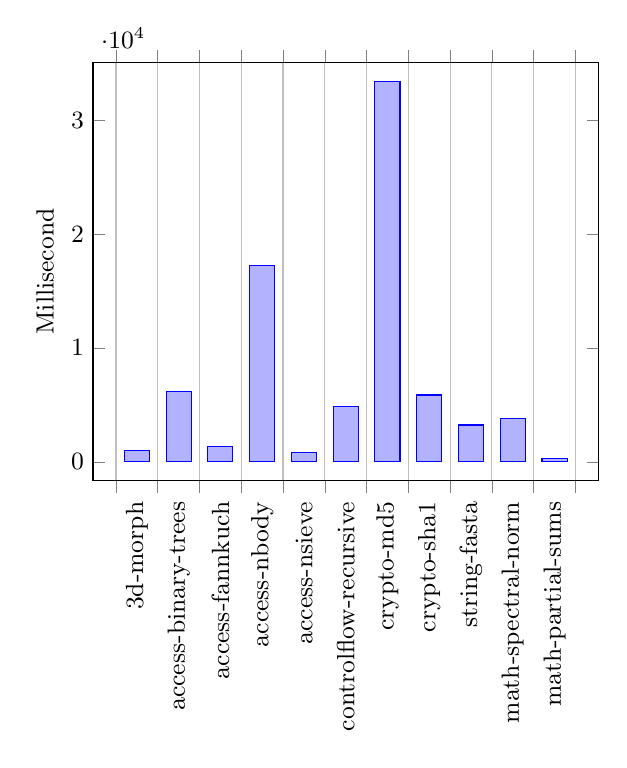
\begin{tikzpicture}
    \pgfplotsset{width=8cm,compat=newest}
    \small
  \begin{axis}[
  	symbolic x coords={3d-morph,access-binary-trees,access-fannkuch,access-nbody,access-nsieve,controlflow-recursive,crypto-md5,crypto-sha1,string-fasta, math-spectral-norm,math-partial-sums,empty},
    xtick=data,
  	ylabel=Millisecond,
  	enlargelimits=0.05,
  	legend style={at={(0.5,-0.33)},
  	anchor=north,legend columns=-1},
  	ybar interval=0.6,
    x tick label style={rotate=90},
  ]
  \addplot
  	coordinates {(3d-morph,989) (access-binary-trees,6165)
  		 (access-fannkuch,1372) (access-nbody,17249) (access-nsieve,790) (controlflow-recursive,4861) (crypto-md5, 33435)
       (crypto-sha1, 5867) (string-fasta, 3235) (math-spectral-norm,3808) (math-partial-sums,306) (empty,0)};
  \end{axis}
  \end{tikzpicture}
  \caption{JsCFA Benchmarks}
  \label{jscfa-benchmark}
\end{figure}

\chapter{Future Work}
\label{sec:Future}
\paragraph{Performance}
The most serious problem of JsCFA is that it uses a naive implementation of AAM framework, which causes the abstract interpreter to slow.
Although AAM provides a systematic approach for constructing correct abstract interpreters easily, the performance is much slower than traditional hand-optimized analyzers.
Therefore, our implementation of JsCFA spends too much time analyzing large-scale programs.
Fortunately, there are several optimizing solutions published for accelerating the computation in AAM\@.
Johnson, Labich, Nicholas, Might, and Van Horn introduced OAAM (optimizing abstracting abstract machine~\cite{johnson2013optimizing}), which is a series of techniques to refine the performance of AAM\@.
This includes timestamped frontier, log-based store deltas, laziness, and abstract compilation that all can dramatically promote AAM in practice or theory.
Thus, in the further research we are going to apply these optimizing techniques for JsCFA\@.

\paragraph{Interface}
Although, \textit{h}-CFA and JsCFA are much easier to implement and understand than traditional abstract interpreters, they still have a common disadvantage that complicates development of static analyzers.
The above described details show that implementing JsCFA is almost similar to writing a concrete interpreter, so programmers can directly convert their compiler or interpreter knowledge to static analysis.
However, \textit{h}-CFA and JsCFA are both based on CESK abstract machine that is a small-step semantic model.
For realistic programming languages that have relatively complex syntax, the implementation of small-step semantics has to introduce many ``continuation'' components.
Manually operating various continuations is tedious, and comparing to big-step operation semantics that makes abstract interpreter code  unintuitive.
Consequently, in the further development we plan to design a domain specific language (DSL) that describes abstract semantics in the big-step style, and abstract interpreters written in the DSL can be compiled to small-step CESK or CESK$^H$ machines.
Olivier discovered a fact in~\cite{danvy2008defunctionalized} that there is an essential connection between big-step operation semantics and small-step CEK machine~\cite{felleisen2009semantics}.
A big-step interpreter can be translated to an equivalent small-step interpreter though CPS transformation~\cite{danvy1992representing}, defunctionalization~\cite{danvy2001defunctionalization}, and fusion.
Therefore, we will continue to design the DSL and the compiler to make abstract interpreters closer to concrete ones.

\paragraph{Precision}
Because JavaScript is a prototype-based highly dynamic programming language that heavily relies upon objects, usually pure control flow analysis is not enough for realistic JavaScript programs and libraries.
Various previous work applies different techniques to analyze JavaScript or subsets of it, such as pointer analysis, string analysis, and numeric range analysis.
JSAI~\cite{kashyap2014jsai} is a static analyzer for JavaScript based on AAM that uses more sophisticated models for abstract objects, abstract strings, and constant propagation.
TAJS~\cite{jensen2009type} is another theory providing a well-designed type system to JavaScript static analysis.
Since objects in JavaScript are maps from strings to values, precise string analysis benefits dynamic extended objects.
Then, object analysis also impacts control flow analysis because methods are fields of objects.
Additionally, arrays are just a kind of special object in JavaScript, a better string/number analysis also improves analysis for arrays.
Consequently, we plan to mix these existing techniques with our control flow analysis solution to increasingly boost JsCFA\@.

\chapter{Conclusion}
\label{sec:Conclude}
We have described \textit{h}-CFA, a simplified approach for implementing pushdown control flow analysis.
This algorithm based on abstracting abstract machine precisely matches returns with calls, which strength is acquired by bringing context (ecording program execution histories) to continuations.
Then, We showed advantages of \textit{h}-CFA comparing with existing pushdown CFA techniques (i.e.\ PDCFA, AAC, P4F).
We designed and implemented JsCFA, a control flow analyzer for JavaScript, which demonstrates that \textit{h}-CFA is a practical approach for realistic programs.
Meanwhile, we discussed the reason why pushdown CFA requires polyvariant continuations to achieve call/return matching, and we used this essential property of pushdown CFA to implement \textit{h}-CFA for JsCFA without recording program execution histories.
In addition, JsCFA adopted other techniques (i.e.\ abstract garbage collection) collaborating with perfect call/return matching to improve the static analysis for JavaScript.
In conclusion, we believe that \textit{h}-CFA can make precise control flow analysis easily implementing for real world programming languages.

\clearpage
\bibliographystyle{plain}
\bibliography{Thesis}
\end{document}
